\documentclass[xcolor=svgnames,9pt,english, aspectratio=169]{beamer}
%\documentclass[xcolor=svgnames,9pt,english, handout, aspectratio=169]{beamer}
\newcommand{\handout}{0}
% Shared template layer for the six decks: theme, beamer layout, and the packages
% every deck needs. Each deck inputs this near the top of its preamble, BEFORE
% ../common/theme.tex (metropolis must be selected before the palette overrides it).
%
% Notation macros and theorem environments are deliberately NOT shared. They
% conflict between the decks, and merging them would silently change symbols
% inside equations:
%   \e          decks 1-2: \bs{\epsilon}      deck 3: \boldsymbol{\eta}
%   \M          decks 1-2: \mb{M}             deck 3: \mathcal{M}
%   \blue       decks 1-2: blue               deck 3: RoyalBlue
%   \indep      different implementations
%   assumption / proposition
%               decks 1-2: own counter        deck 3: shares the theorem counter
%
% Each deck therefore keeps its own notation block. Only the look is unified.

\usetheme{metropolis}
\setbeamertemplate{navigation symbols}{}

% Deck 3's margins; decks 1 and 2 previously used 2em, which at 9pt is ~6.3mm.
\setbeamersize{text margin left=5mm, text margin right=5mm}
\setbeamertemplate{itemize/enumerate body begin}{\leftmargini=1.5em\relax}
\setbeamertemplate{itemize/enumerate subbody begin}{\leftmarginii=1.5em\relax}
\setbeamertemplate{itemize/enumerate subsubbody begin}{\leftmarginiii=1.5em\relax}

\usepackage{xcolor}
\usepackage{colortbl}
\usepackage{amsmath}
\usepackage{amsfonts}
\usepackage{amssymb}
\usepackage{graphicx}
\usepackage{multirow}
\usepackage{listings}
\usepackage{booktabs}
\usepackage{tikz}
\usetikzlibrary{arrows.meta,positioning,decorations.pathreplacing}

% Citations: one bib file at the repository root, Chicago author-date via biblatex-chicago
% (needs biber). Reference frames are generated with \printbibliography; in-text citations
% use \textcite (narrative) and \parencite (parenthetical). The CMS rule prints one to three
% names in full and four or more as "First et al."; \citeshort forces "et al.", \citeall
% prints every name (text/paren/author variants likewise). The override lasts one citation.
\usepackage{csquotes}
\usepackage[authordate,backend=biber,doi=false,url=false,isbn=false,eprint=false,
            maxbibnames=10,compresspages=true,dashed=false]{biblatex-chicago}
\addbibresource{../references.bib}
% Entry size: beamer wraps each part of a biblatex entry in its "bibliography entry author /
% title / location / note" fonts, and metropolis sets those to \normalsize, so \bibfont alone
% does not change the size. The four \setbeamerfont lines in theme.tex set the size that shows.
\renewcommand*{\bibfont}{\scriptsize}
\setlength{\bibitemsep}{0.7em}   % visible air between entries
\setlength{\bibhang}{0.5em}
% The References frame of every deck: \begin{frame}[t,allowframebreaks=1.0] ... \referencelist.
% Beamer's automatic break for this list fires at about two thirds of the frame; the factor
% 1.1 lets it fill the frame. The small negative skip closes the list's top gap.
\newcommand{\referencelist}{\vspace*{-0.6em}\printbibliography[heading=none]}
\newcommand{\citeshort}[1]{\AtNextCitekey{\defcounter{maxnames}{1}}\cite{#1}}
\newcommand{\textciteshort}[1]{\AtNextCitekey{\defcounter{maxnames}{1}}\textcite{#1}}
\newcommand{\parenciteshort}[1]{\AtNextCitekey{\defcounter{maxnames}{1}}\parencite{#1}}
\newcommand{\citeauthorshort}[1]{\AtNextCitekey{\defcounter{maxnames}{1}}\citeauthor{#1}}
\newcommand{\citeall}[1]{\AtNextCitekey{\defcounter{maxnames}{9}}\cite{#1}}
\newcommand{\textciteall}[1]{\AtNextCitekey{\defcounter{maxnames}{9}}\textcite{#1}}
\newcommand{\parenciteall}[1]{\AtNextCitekey{\defcounter{maxnames}{9}}\parencite{#1}}
% PDF metadata: beamer copies the whole \author box into the author field; set it plainly
% once every deck-level \author has run (etoolbox's end-of-preamble hook).
\AtEndPreamble{\hypersetup{pdfauthor={Yiqing Xu}}}
   % theme, layout, packages

\setbeamertemplate{footline}[frame number]{}

\graphicspath{{./figs/}}%
\newcommand{\red}{\textcolor{red}}

% Beamer margin


\usepackage{epsfig}
% Shared visual system for the six decks: palette, fonts, footline.
% Swap the four colors below to rebrand every deck at once.
\definecolor{SlideRed}{HTML}{9E1B32}
\definecolor{SlideInk}{HTML}{252A34}
\definecolor{SlideBlue}{HTML}{2F6B9A}
\definecolor{SlideMist}{HTML}{F8F3F3}


\setbeamercolor{normal text}{fg=SlideInk,bg=white}
\setbeamercolor{structure}{fg=SlideRed}
\setbeamercolor{alerted text}{fg=SlideRed}
\setbeamercolor{frametitle}{fg=white,bg=SlideRed}
\setbeamercolor{title}{fg=SlideRed}
\setbeamercolor{subtitle}{fg=SlideInk}
\setbeamercolor{block title}{fg=white,bg=SlideRed}
\setbeamercolor{block body}{fg=SlideInk,bg=SlideMist}
\setbeamercolor{section in toc}{fg=SlideRed}

\setbeamerfont{title}{series=\bfseries,size=\Large}
\setbeamerfont{frametitle}{series=\bfseries,size=\large}
\setbeamerfont{block title}{series=\bfseries}
\setbeamertemplate{navigation symbols}{}
\setbeamertemplate{items}[circle]
\setbeamertemplate{blocks}[rounded][shadow=false]
\setbeamertemplate{bibliography item}{}   % no document icons on the References frames
\setbeamertemplate{frametitle continuation}{}
\setbeamertemplate{footline}{%
  \leavevmode\hbox{%
  \begin{beamercolorbox}[wd=.88\paperwidth,ht=2.6ex,dp=1.2ex,leftskip=1.2em]{author in head/foot}%
  \usebeamerfont{author in head/foot}\insertshorttitle
  \end{beamercolorbox}%
  \begin{beamercolorbox}[wd=.12\paperwidth,ht=2.6ex,dp=1.2ex,center]{date in head/foot}%
  \insertframenumber
  \end{beamercolorbox}}}

\newcommand{\slidesource}[1]{\vfill{\scriptsize\color{gray}Source: #1}}
\newcommand{\keyquestion}[1]{\begin{block}{Question}#1\end{block}}

% NOTE: do NOT set title/subtitle to white-on-SlideRed here. That relied on Madrid
% filling the title box; metropolis does not, so white text lands on white and the
% title vanishes. ../common/theme.tex already sets title fg=SlideRed, subtitle fg=SlideInk.
%\usepackage{rotating}
%\usepackage{theorem}


% Use the R versions of all software demonstrations.
\newcommand{\solutions}{0}


\title{Panel Methods (1): The Parametric Approach}
\subtitle{Lectures on Causal Panel Analysis}
\author{Yiqing Xu\\\smallskip Stanford University}
\date{September 2026}


%\date[November 2004]{November 26, 2004}

\definecolor{dgreen}{rgb}{0,.6,0.8}
\newtheorem{assumption}{Assumption}
\newtheorem{iass}{Identification Assumption}
\newtheorem{ires}{Identification Result}
\newtheorem{estm}{Estimand}
\newtheorem{esti}{Estimator}
\newtheorem{question}{Question}
\newtheorem{answer}{Answer}
\newtheorem{proposition}{Proposition}
\newcommand{\bs}{\boldsymbol}
\newcommand{\mb}{\mathbf}
\newcommand{\real}{\mathbb{R}}
\renewcommand{\u}{\ensuremath{\mb{u}}}
\renewcommand{\v}{\ensuremath{\mb{v}}}
\newcommand{\U}{\ensuremath{\mb{U}}}
\newcommand{\M}{\ensuremath{\mb{M}}}
\newcommand{\X}{\ensuremath{\mb{X}}}
\newcommand{\x}{\ensuremath{\mb{x}}}
\newcommand{\y}{\ensuremath{\mb{y}}}
\renewcommand{\b}{\ensuremath{\bs{\beta}}}
\newcommand{\e}{\ensuremath{\bs{\epsilon}}}
\newcommand{\bhat}{\ensuremath{\hat{\bs{\beta}}}}
\newcommand{\XX}{\ensuremath{\X'\X}}
\newcommand{\XXinv}{\ensuremath{\left(\XX\right)^{-1}}}
\newcommand{\hatsig}{\ensuremath{\hat{\sigma}^2}}
\newcommand{\sig}{\ensuremath{\sigma^2}}
\newcommand{\hatmat}{\ensuremath{\X \XXinv \X'}}
\newcommand{\ehat}{\ensuremath{\hat{\e}}}
\newcommand{\tr}{\text{tr}}
\newcommand{\Sig}{\ensuremath{\bs{\Sigma}}}
\newcommand{\SigInv}{\ensuremath{\bs{\Sigma^{-1}}}}
\newcommand{\W}{\ensuremath{\mb{W}}}

\newcommand{\indep}{{\bot\negthickspace\negthickspace\bot}}
% Shared workshop theme supplies the minimal footline.


\begin{document}

\subject{Talks}
\AtBeginSection[]
{
  \begin{frame}
    \frametitle{Lecture 1 Roadmap}
    \tableofcontents[currentsection]
  \end{frame}
}

\AtBeginSubsection[]
{
  \begin{frame}
    \frametitle{Lecture 1 Roadmap}
    \tableofcontents[currentsection,currentsubsection]
  \end{frame}
}

\begin{frame}
  \titlepage
  \thispagestyle{empty}
  \addtocounter{framenumber}{-1}
\end{frame}


\frame{
\frametitle{Motivations}
\begin{itemize}\itemsep0.3em
\item Causal inference is challenging with observational data\pause
\item Panel data often come to the rescue (\alert{false hope?})\pause
\item In the social sciences, difference-in-differences (DiD) and two-way fixed effects (TWFE) are the most popular
\end{itemize}
\begin{center}
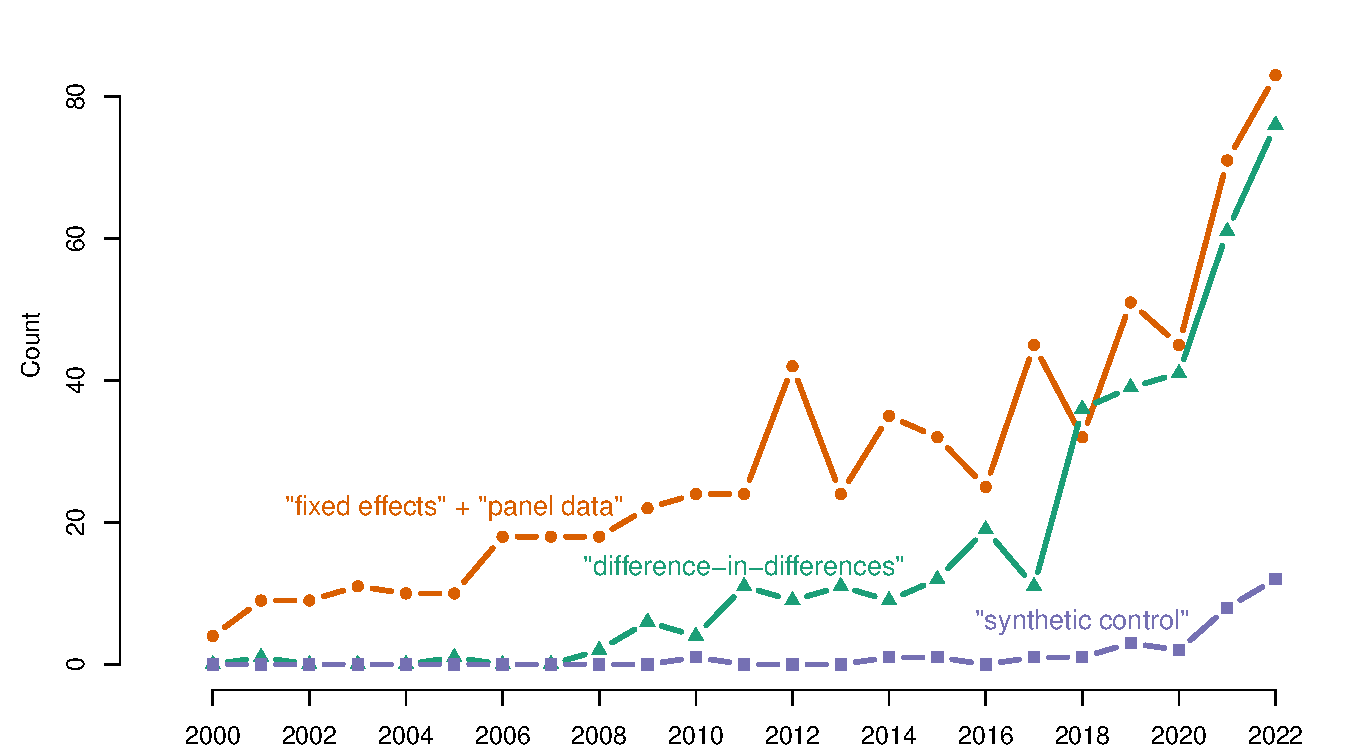
\includegraphics[scale = 0.4]{journal.pdf}
\end{center}
}

\begin{frame}
  \frametitle{What's a Panel Dataset?}
\begin{center}
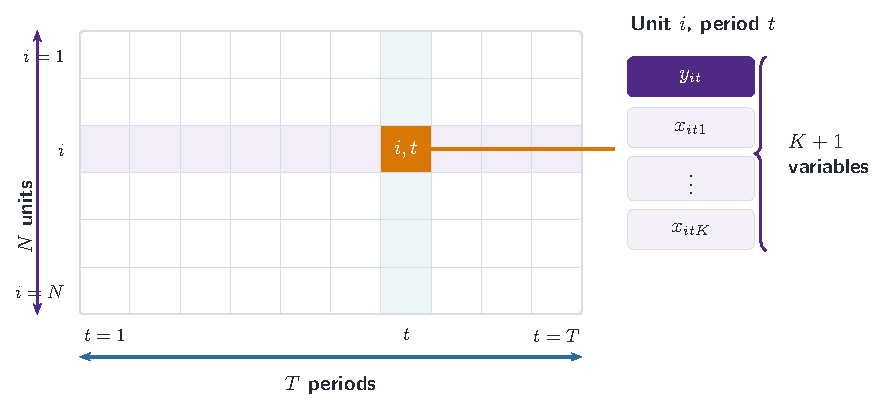
\includegraphics[width=0.94\textwidth,height=0.78\textheight,keepaspectratio]{panel_dataset_sleek_2026.pdf}
\end{center}
\end{frame}  

\begin{frame}
  \frametitle{What's a Panel Dataset?}
\begin{center}
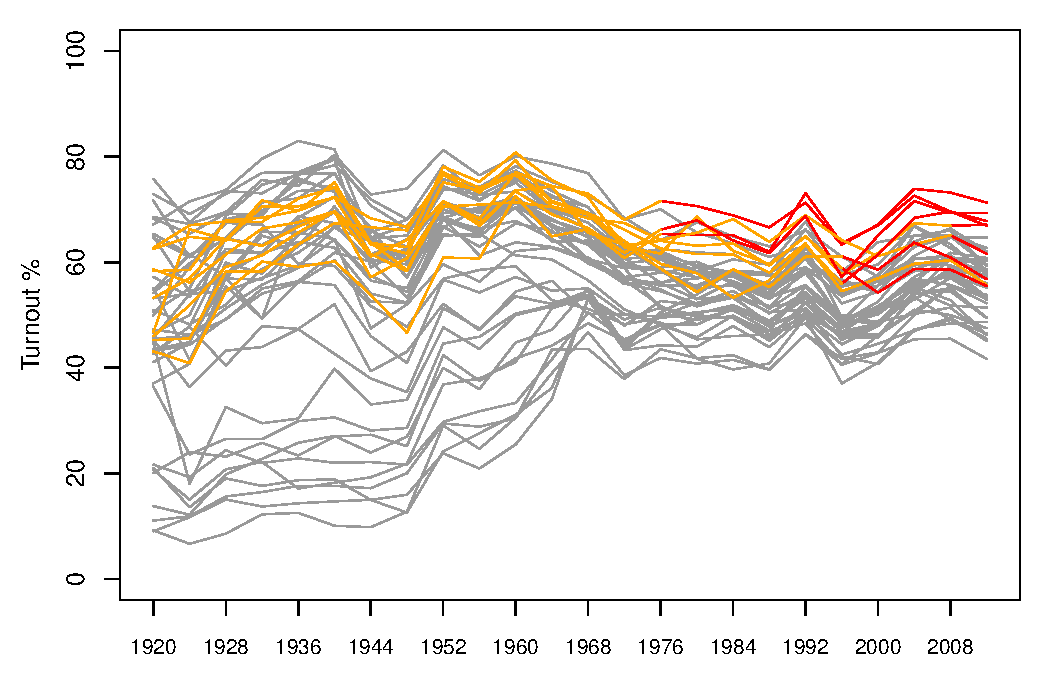
\includegraphics[height = 0.8\textheight]{edr_rawdata.pdf}
\end{center}
\end{frame}  


\if\handout1
\begin{frame}
  \frametitle{What's Causal Inference with Panel Data?}
What would happen if a group of units experienced a set of counterfactual treatment histories?
\begin{center}
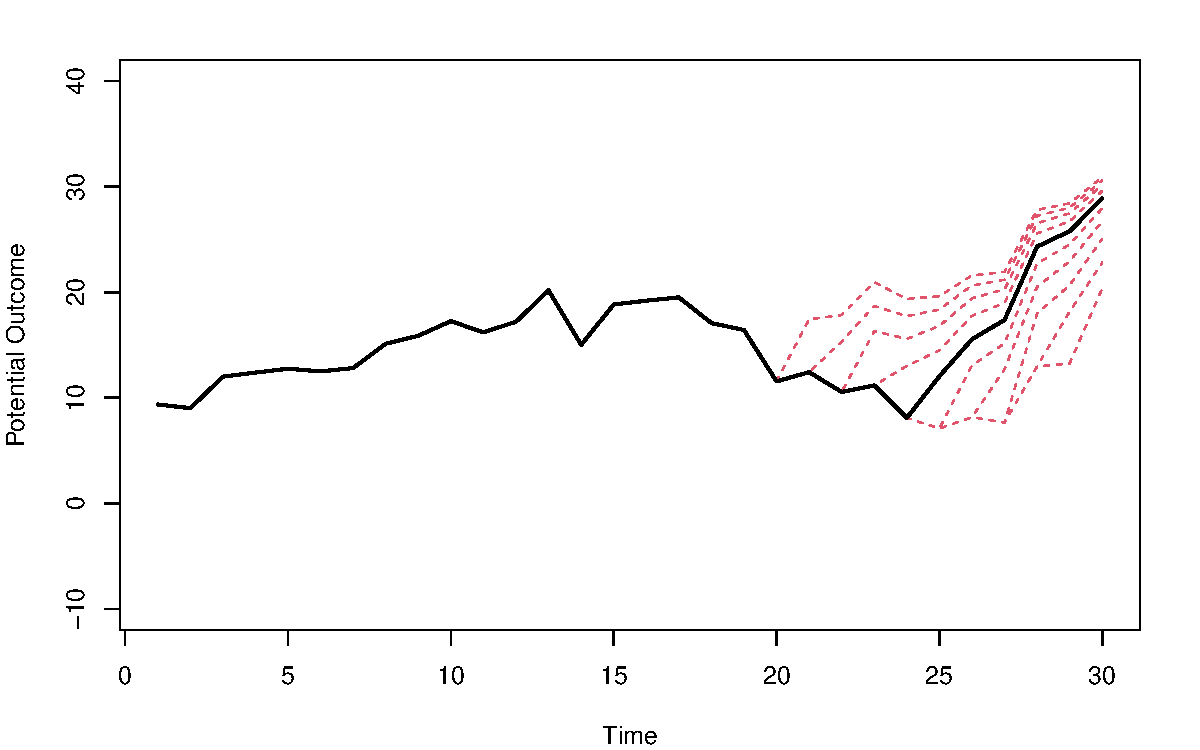
\includegraphics[height = 0.8\textheight]{seq1.pdf}%
\end{center}
\end{frame}  
\fi

\if\handout0
\begin{frame}
  \frametitle{What's Causal Inference with Panel Data?}
What would happen if a group of units experienced a set of counterfactual treatment histories?
\begin{center}
\only<1>{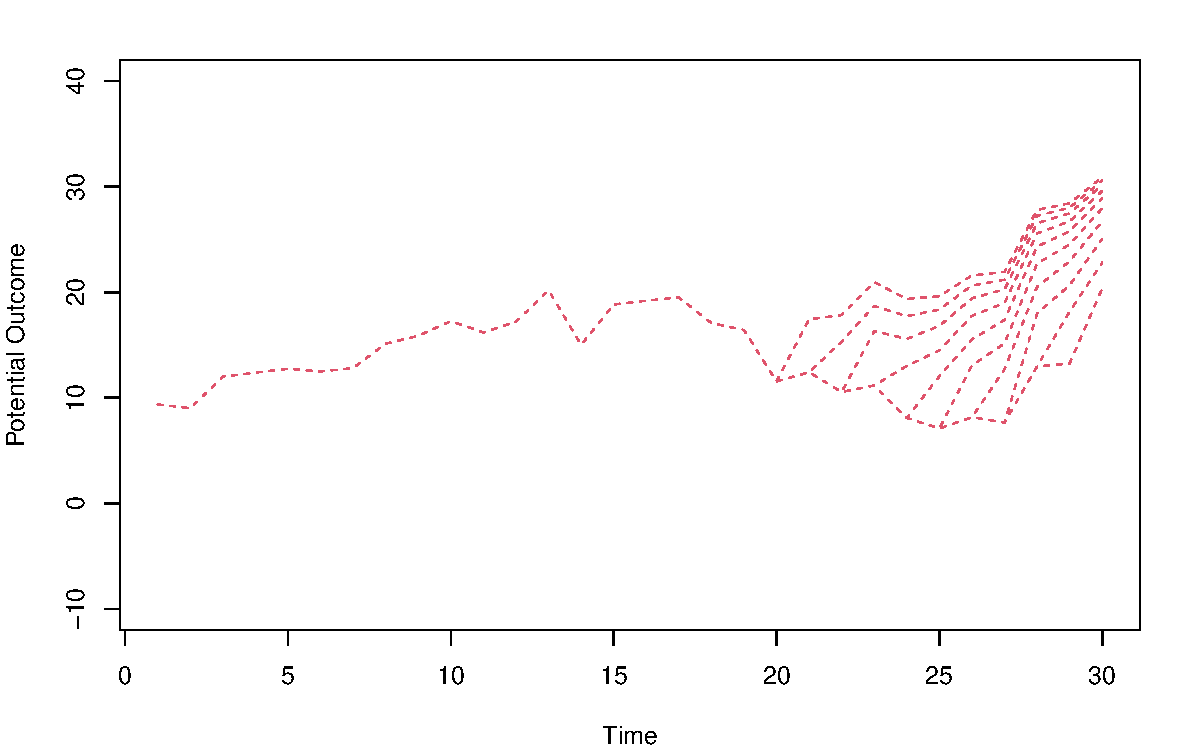
\includegraphics[height = 0.8\textheight]{seq0.pdf}}%
\only<2>{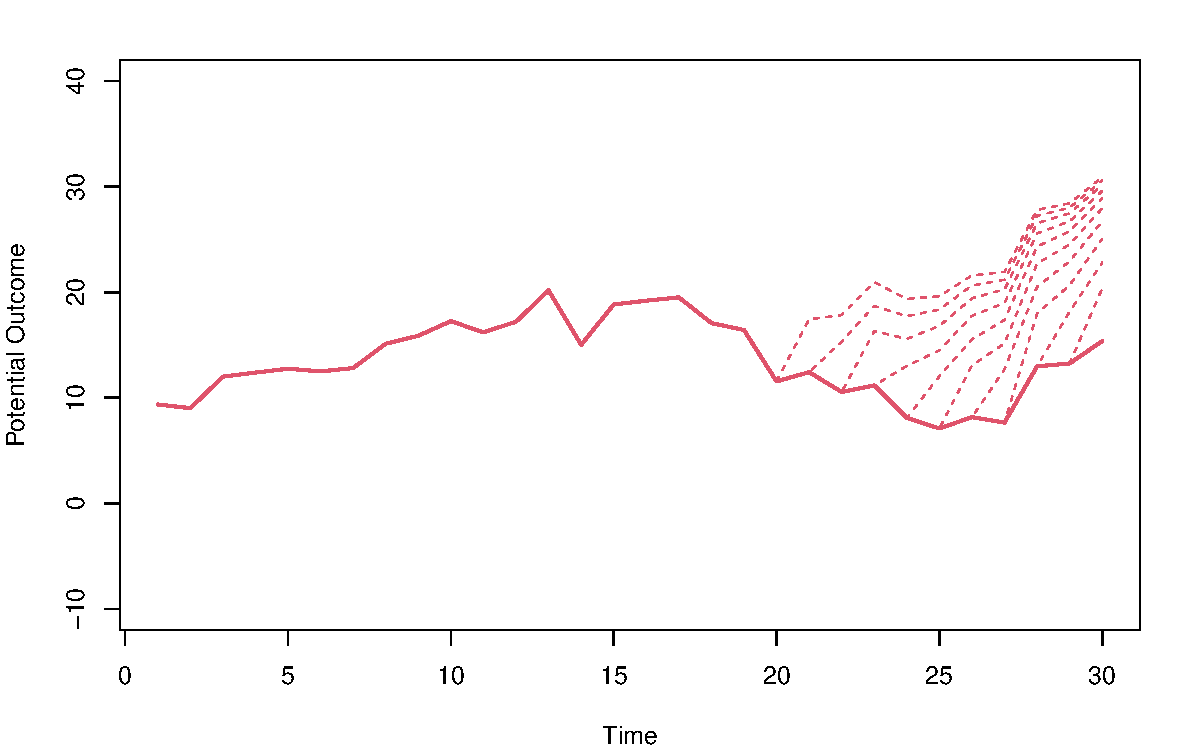
\includegraphics[height = 0.8\textheight]{seq2.pdf}}%
\only<3>{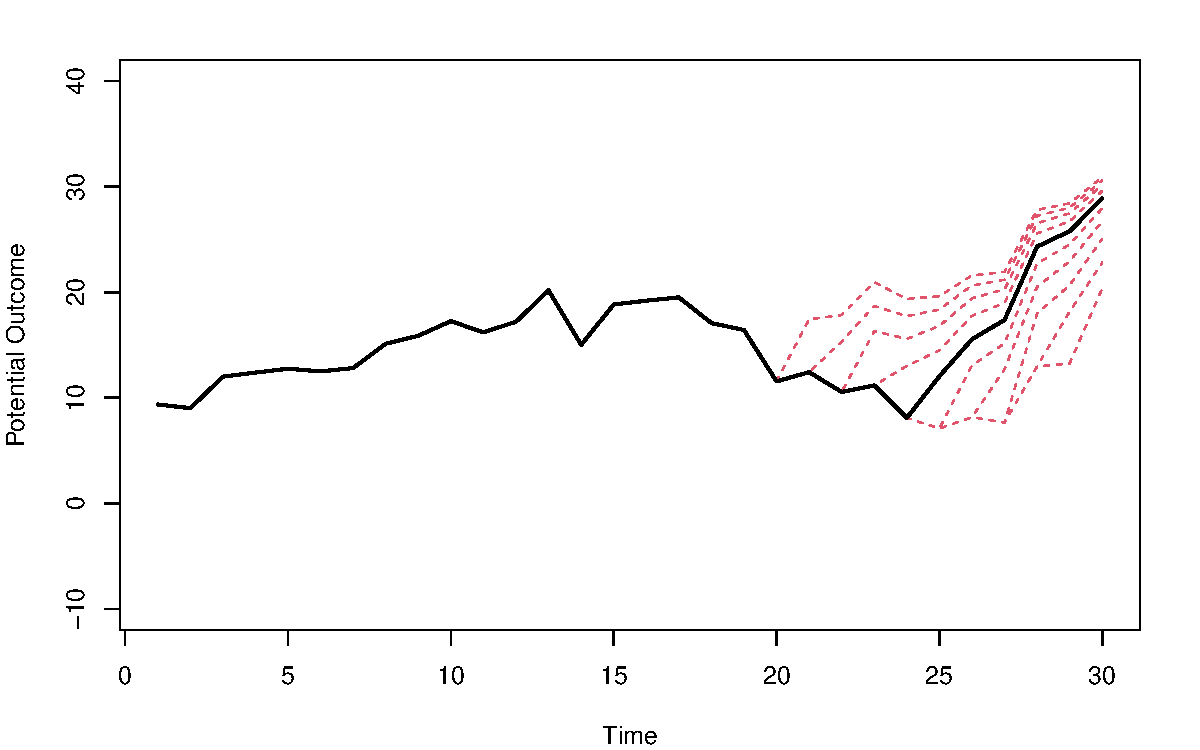
\includegraphics[height = 0.8\textheight]{seq1.pdf}}%
\end{center}
\end{frame}  
\fi


\begin{frame}
  \frametitle{What's Special about Panel Data?}
\begin{itemize}
\item The fundamental problem of causal inference \parencite{holland1986statistics}
\begin{center}
$\tau_{i}=Y_{1i}- Y_{i0}$
\end{center}\pause
\item A \underline{statistical} solution makes use of others' information\\
\begin{center}
e.g. $ATE= E[Y_1]- E[Y_0]$
\end{center}\pause
\item A \underline{scientific} solution exploits homogeneity or invariance assumptions\\
\begin{center}
e.g. The long-run growth rate of the US economy is 2.5\%.
\end{center}\pause
\vspace{0.5cm}
\item Panel data \pause allow us to construct treated counterfactuals using information from both \alert{the past} and \alert{the others} \pause with the caveat that treatment assignment mechanism may be complicated\pause
\item Causal inference with panel data is also challenging because of\pause
\begin{itemize}[<+->]
  \item potentially (very) high dimensional treatment
  \item limited knowledge about treatment assignment mechanisms
  \item both cross-sectional and temporal interference (SUTVA violations)
\end{itemize}
\end{itemize}
\end{frame}

\begin{frame}
  \frametitle{Panel Models Impute Different Counterfactuals}
\begin{center}
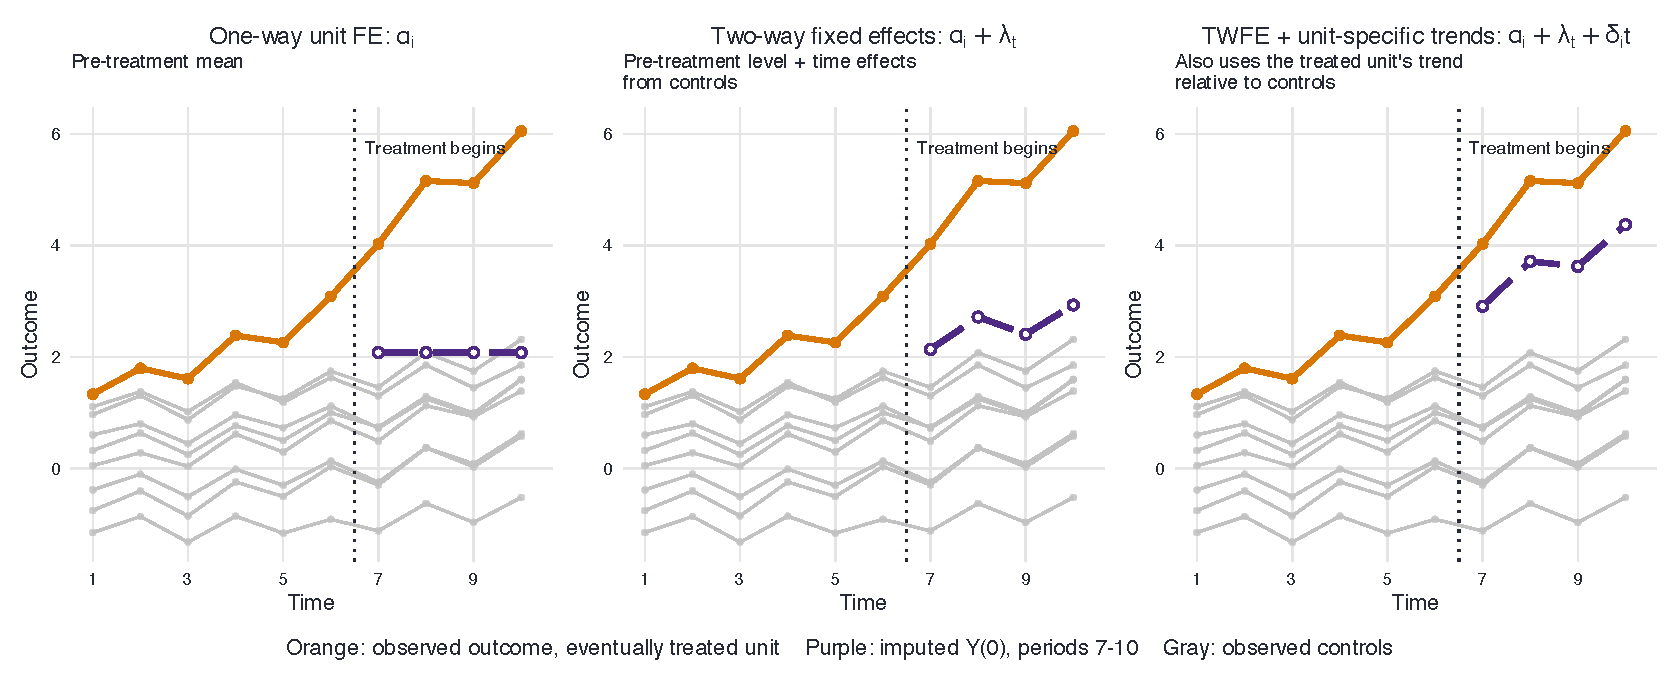
\includegraphics[width=0.98\textwidth]{counterfactual_imputation_models_2026.pdf}
\end{center}
\vspace{-0.4em}
\begin{itemize}\itemsep0.25em
\item<2-> Each fit uses all control outcomes and the treated unit through period 6.
\end{itemize}
\slidesource{Author's simulation.}
\end{frame}


\begin{frame}
  \frametitle{Six Lectures on Panel Methods}
\begin{center}
\begin{tikzpicture}[
  lecture/.style={rounded corners=3pt, draw=SlideRed, thick,
                  minimum height=1.6cm, text width=2.6cm,
                  align=center, inner sep=5pt},
  link/.style={-{Latex[length=2.2mm]}, thick, draw=SlideInk}
]
\node[lecture, fill=SlideRed!10] (l1) at (0,0)
  {\textbf{1. Parametric panel models}\\[0.25em]
   \footnotesize FE regressions and their assumptions};
\node[lecture, fill=SlideBlue!10] (l2) at (0,-2.9)
  {\textbf{2. Difference-in-differences}\\[0.25em]
   \footnotesize The canonical design and identification};
\node[lecture, fill=SlideBlue!10] (l3) at (3.9,0)
  {\textbf{3. Factorial DID}\\[0.25em]
   \footnotesize When the event affects everyone};
\node[lecture, fill=SlideBlue!10] (l4) at (3.9,-2.9)
  {\textbf{4. TWFE revisited}\\[0.25em]
   \footnotesize What breaks under staggered timing};
\node[lecture, fill=SlideBlue!10] (l5) at (7.8,0)
  {\textbf{5. Modern DID}\\[0.25em]
   \footnotesize Heterogeneity-robust estimators};
\node[lecture, fill=SlideRed!10] (l6) at (7.8,-2.9)
  {\textbf{6. Synthetic control \& factor models}\\[0.25em]
   \footnotesize Imputing treated counterfactuals};
\draw[link] (l1) -- (l2);
\draw[link] (l2.east) -- ++(0.5,0) |- (l3.west);
\draw[link] (l3) -- (l4);
\draw[link] (l4.east) -- ++(0.5,0) |- (l5.west);
\draw[link] (l5) -- (l6);
\end{tikzpicture}
\end{center}
\vspace{0.1em}\pause
\centering\small Lectures 1 and 6 build counterfactuals from outcome models; the rest start from treatment-timing comparisons, with assumptions tailored to those comparisons.
\end{frame}

\begin{frame}
  \frametitle{Lecture 1 Roadmap}
\begin{center}
\begin{tikzpicture}[
  roadmapbox/.style={rounded corners=3pt, draw=SlideRed, thick,
               minimum height=1.55cm, text width=2.55cm,
               align=center, fill=SlideRed!7},
  link/.style={-{Latex[length=2.2mm]}, thick, draw=SlideInk}
]
\node[roadmapbox] (s1) at (0,0) {Panel setup\\and confounding};
\node[roadmapbox] (s2) at (3.7,0) {Pooled OLS, FE,\\and RE};
\node[roadmapbox] (s3) at (7.4,0) {Common time effects\\and unit trends};
\node[roadmapbox] (s4) at (11.1,0) {Dynamic and\\heterogeneous effects};
\draw[link] (s1) -- (s2);
\draw[link] (s2) -- (s3);
\draw[link] (s3) -- (s4);
\end{tikzpicture}
\end{center}
\bigskip\pause
\begin{block}{Main question}
Which observations does each estimator compare, and under what conditions does that comparison recover a causal effect?
\end{block}
\end{frame}

\begin{frame}
  \frametitle{Application 1: Direct Democracy and Naturalization}
\begin{columns}[T,onlytextwidth]
\begin{column}{0.47\textwidth}
\centering
\textbf{Treatment timing}\par\smallskip
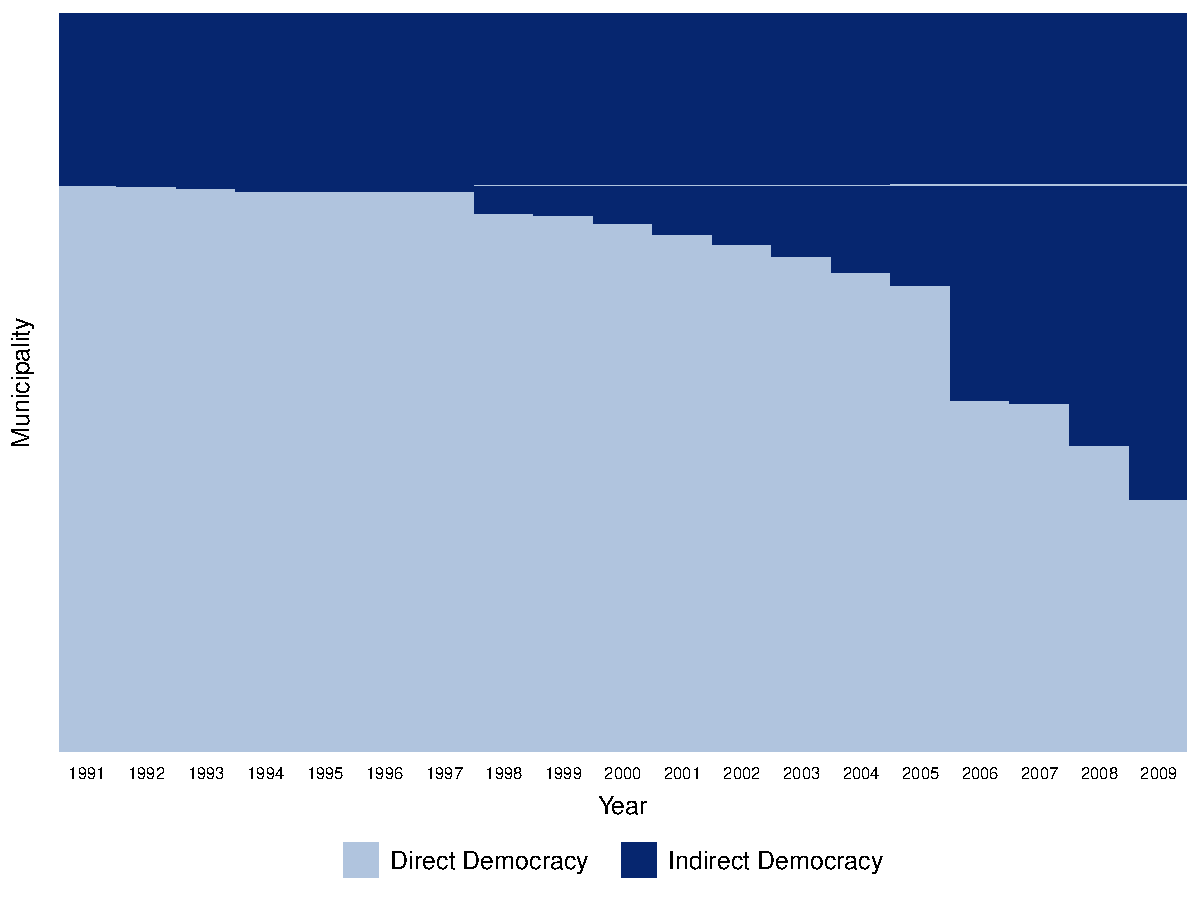
\includegraphics[width=\linewidth,height=0.49\textheight,keepaspectratio]{ex_HH2015_treat.pdf}
\end{column}
\begin{column}{0.50\textwidth}
\centering
\onslide<2->{\textbf{Naturalization rates in six municipalities}\par\smallskip
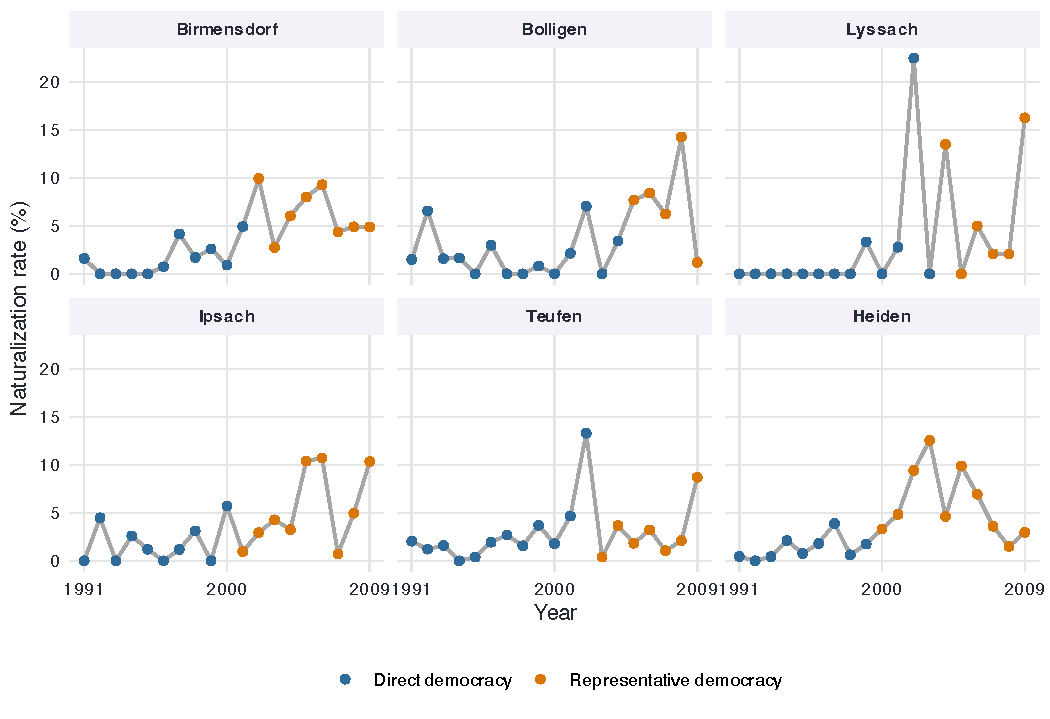
\includegraphics[width=\linewidth,height=0.49\textheight,keepaspectratio]{naturalization_intro_2026.pdf}}
\end{column}
\end{columns}
\vspace{0.2em}
\onslide<3->{\keyquestion{Do elected municipal councils raise naturalization rates relative to citizen referendums?}}
\slidesource{\textcite{hainmueller2019direct}.}
\end{frame}

\begin{frame}
  \frametitle{Application 2: Beer Taxes and Fatalities}
\begin{columns}[T,onlytextwidth]
\begin{column}{0.49\textwidth}
\centering
\textbf{Pooled comparison}\par\smallskip
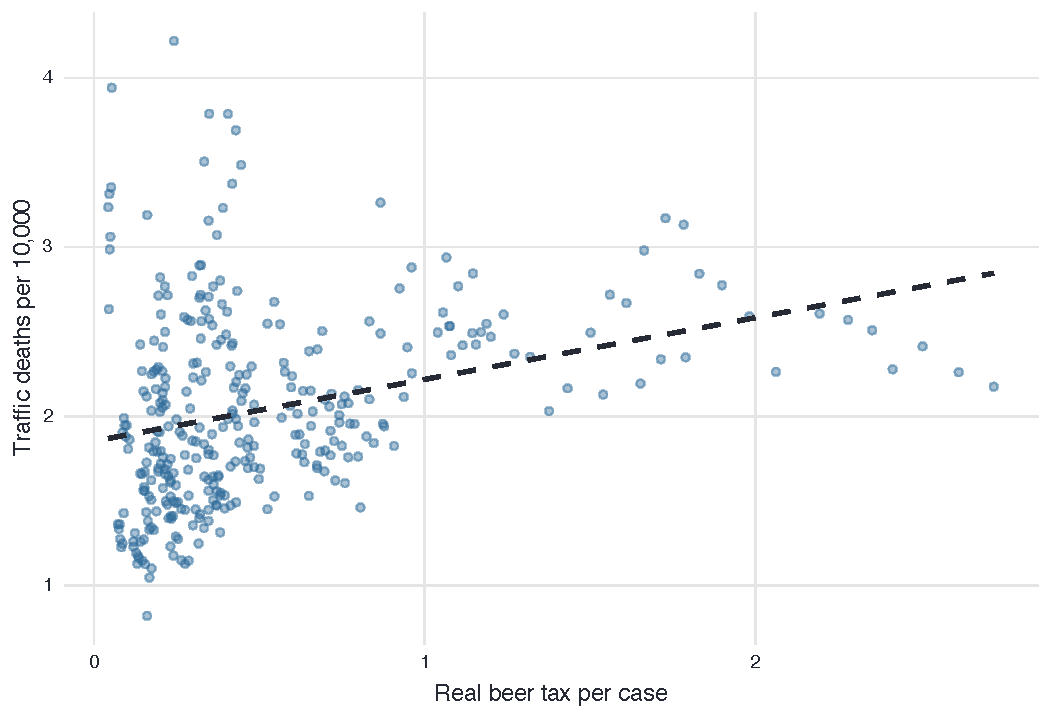
\includegraphics[width=\linewidth,height=0.49\textheight,keepaspectratio]{fatalities_intro_2026.pdf}
\end{column}
\begin{column}{0.49\textwidth}
\centering
\onslide<2->{\textbf{After subtracting each state's mean}\par\smallskip
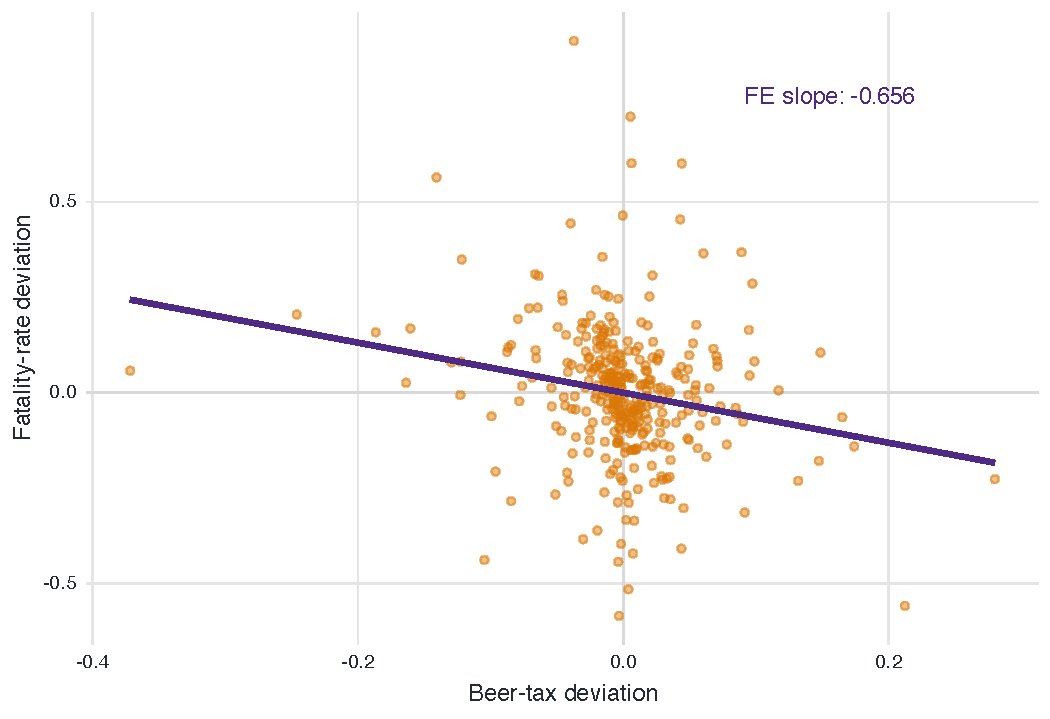
\includegraphics[width=\linewidth,height=0.49\textheight,keepaspectratio]{fatalities_within_2026.pdf}}
\end{column}
\end{columns}
\vspace{0.1em}
\onslide<3->{\keyquestion{Do higher beer taxes reduce traffic fatalities?}}
\slidesource{\textcite{ruhm1996alcohol}; \textcite{stock2007introduction}.}
\end{frame}

\section{Panel Setup \& Unobserved Confounding}


\begin{frame}
\small
  \frametitle{Panel Setup}
Single unit: $$
\y_i = \left(
  \begin{array}{c}
    y_{i1} \\
     \vdots\\
    y_{it} \\
    \vdots \\
    y_{iT} \\
  \end{array}
\right)_{T \times 1} \qquad  \X_i = \left(
  \begin{array}{cccccc}
    x_{i,1,1} & x_{i,1,2} & x_{i,1,j} & \dotsb &  x_{i,1,K} \\
     \vdots & \vdots & \vdots & & \vdots\\
   x_{i,t,1} & x_{i,t,2} & x_{i,t,j} & \dotsb &  x_{i,t,K} \\
   \vdots & \vdots & \vdots & & \vdots\\
   x_{i,T,1} & x_{i,T,2} & x_{i,T,j} & \dotsb &  x_{i,T,K} \\
  \end{array}
\right)_{T \times K}
$$
Panel with all units: $$
\y = \left(
  \begin{array}{c}
    \y_{1} \\
     \vdots\\
    \y_{i} \\
    \vdots \\
    \y_{N} \\
  \end{array}
\right)_{NT \times 1} \qquad  \X = \left(
  \begin{array}{c}
    \X_{1} \\
     \vdots\\
    \X_{i} \\
    \vdots \\
   \X_{N} \\
  \end{array}
\right)_{NT \times K}
$$
\end{frame}


\begin{frame}
  \frametitle{Unobserved Effects Model: Farm Output}
\small
\begin{itemize}
\item For a randomly drawn cross-sectional unit $i$, the model is given by
\[
y_{it} = \x_{it}\b + c_i + \varepsilon_{it}, \quad \quad t=1,2,...,T
\]\vspace{-.2in}
%\item Example:
\begin{itemize}[<+->]
  \item $y_{it}$: output of farm $i$ in year $t$\medskip
  \item $\x_{it}$: $1 \times K$ vector of variable inputs  for farm $i$ in year $t$, such as labor, fertilizer, etc. plus an intercept\medskip
  \item \red{$\b$}:  $K \times 1$ vector of marginal effects of variable inputs, the \red{causal quantity of interest}\medskip
  \item $c_i$: farm effect, i.e. the sum of all time-invariant inputs known to farmer $i$ (but unobserved for the researcher), such as soil quality, managerial ability, etc.
  \begin{itemize}
  \item often called: \alert{unobserved effect}, \alert{unobserved heterogeneity}, capturing \red{unobserved confounding}
\end{itemize}\medskip
\item $\varepsilon_{it}$: time-varying unobserved inputs, such as rainfall, unknown to the farmer
at the time the decision on the variable inputs $\x_{it}$ is made
\begin{itemize}
  \item often called: \alert{idiosyncratic error}
\end{itemize}
\end{itemize}\pause
\item What happens when we regress $y_{it}$ on $\x_{it}$?
\end{itemize}
\end{frame}

\begin{frame}
  \frametitle{Pooled OLS}
  \small
\begin{itemize}
\item When we ignore the panel structure and regress $y_{it}$ on $\x_{it}$ we get
\[
y_{it} = \x_{it}\b + v_{it}, \quad \quad t=1,2,...,T
\]
with \alert{composite error} $v_{it} \equiv c_i + \varepsilon_{it}$\medskip
\item Main assumption to obtain consistent estimates for $\b$ is:\medskip\pause
 \begin{itemize}
   \item $E[v_{it}|\x_{i1},\x_{i2},...,\x_{iT}]=E[v_{it}|\x_{it}]=0$ for $t=1,2,...,T$
   \begin{itemize}
    \item $\x_{it}$ are \alert{strictly exogenous}: the composite error $v_{it}$ in each time period is uncorrelated with the past, current, and future regressors
    \item But: labour input $\x_{it}$ likely depends on soil quality $c_i$ and so we have omitted variable bias and $\bhat$ is not consistent
%    rules out omitted variables, lagged effects, and feedback
    \end{itemize}\medskip\pause
 \item No correlation between $\x_{it}$ and $v_{it}$ $\Rightarrow$ no correlation between unobserved effect $c_{i}$ and $\x_{it}$ for all $t$
 \begin{itemize}
   \item Violations are common: whenever we omit a time-constant variable that is correlated with the regressors (\alert{unoberseved confounding})
 \end{itemize}
%\item Additional problem: $v_{it}$ are serially correlated for same $i$ since $c_i$ is present in each $t$ and thus pooled OLS standard errors are invalid
 \end{itemize}
\end{itemize}
\end{frame}

\begin{frame}
  \frametitle{Unobserved Effects Model: Program Evaluation}
  \small
\begin{itemize}
\item Program evaluation model:
\[
y_{it} = prog_{it}\,\b + c_i + \varepsilon_{it}, \quad \quad t=1,2,...,T
\]\vspace{-.2in}
\begin{itemize}
  \item $y_{it}$: log wage of individual $i$ in year $t$\medskip
  \item $prog_{it}$: indicator coded 1 if individual $i$ participants in training program at $t$ and 0 otherwise\medskip
  \item $\b$: \red{effect of program}\medskip
  %\item $\x_{it}$ other individual characteristics that affect wages (and intercept)
  \item $c_i$: sum of all time-invariant unobserved characteristics that affect wages, such as ability, etc.
\end{itemize}\pause
\item What happens when we regress $y_{it}$ on $prog_{it}$? \pause $\bhat$ not consistent since $prog_{it}$ is likely correlated with $c_i$ (e.g. ability)\medskip\pause
\item Always ask: Is there a time-constant unobserved variable ($c_i$) that is correlated with the regressors? If yes, pooled OLS is problematic\pause
\item Additional problem: $v_{it} \equiv c_i + \varepsilon_{it}$ are serially correlated for same $i$ since $c_i$ is present in each $t$ and thus pooled OLS standard errors are invalid
\end{itemize}
\end{frame}


\section{Fixed Effects Regression}

\begin{frame}
  \frametitle{Simpson's Paradox: Pooled and Within-State Slopes}
\begin{center}
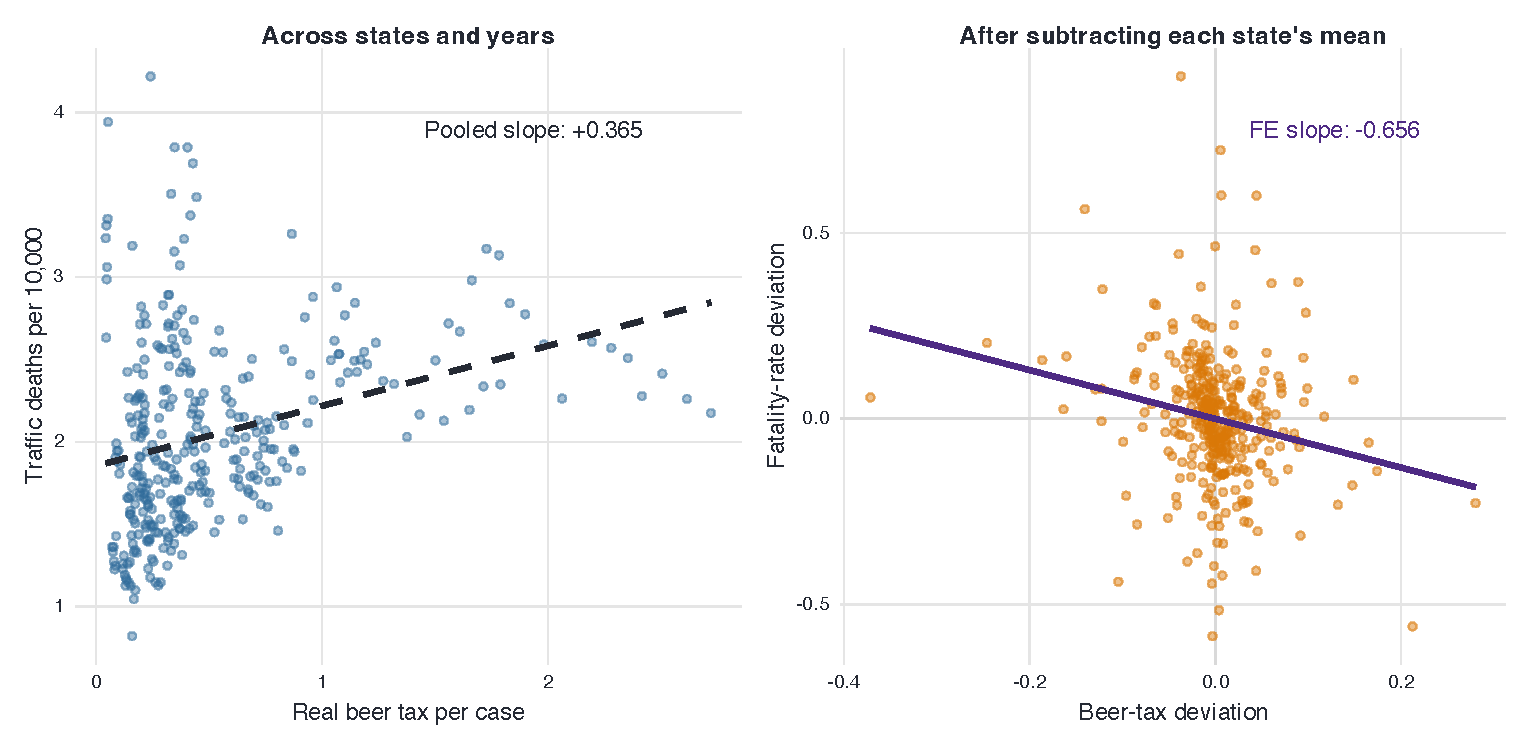
\includegraphics[height=0.64\textheight]{simpson_fe_2026.pdf}
\end{center}
\vspace{-0.5em}
\begin{itemize}\itemsep0.25em
\item<2-> Each dot is a state-year observation.
\item<3-> Subtracting each state's means changes the slope from $+0.365$ to $-0.656$.
\end{itemize}
\slidesource{U.S. traffic-fatality panel; \textcite{ruhm1996alcohol} and \textcite{stock2007introduction}.}
\end{frame}

\begin{frame}
  \frametitle{Between-State and Within-State Variation}
\begin{center}
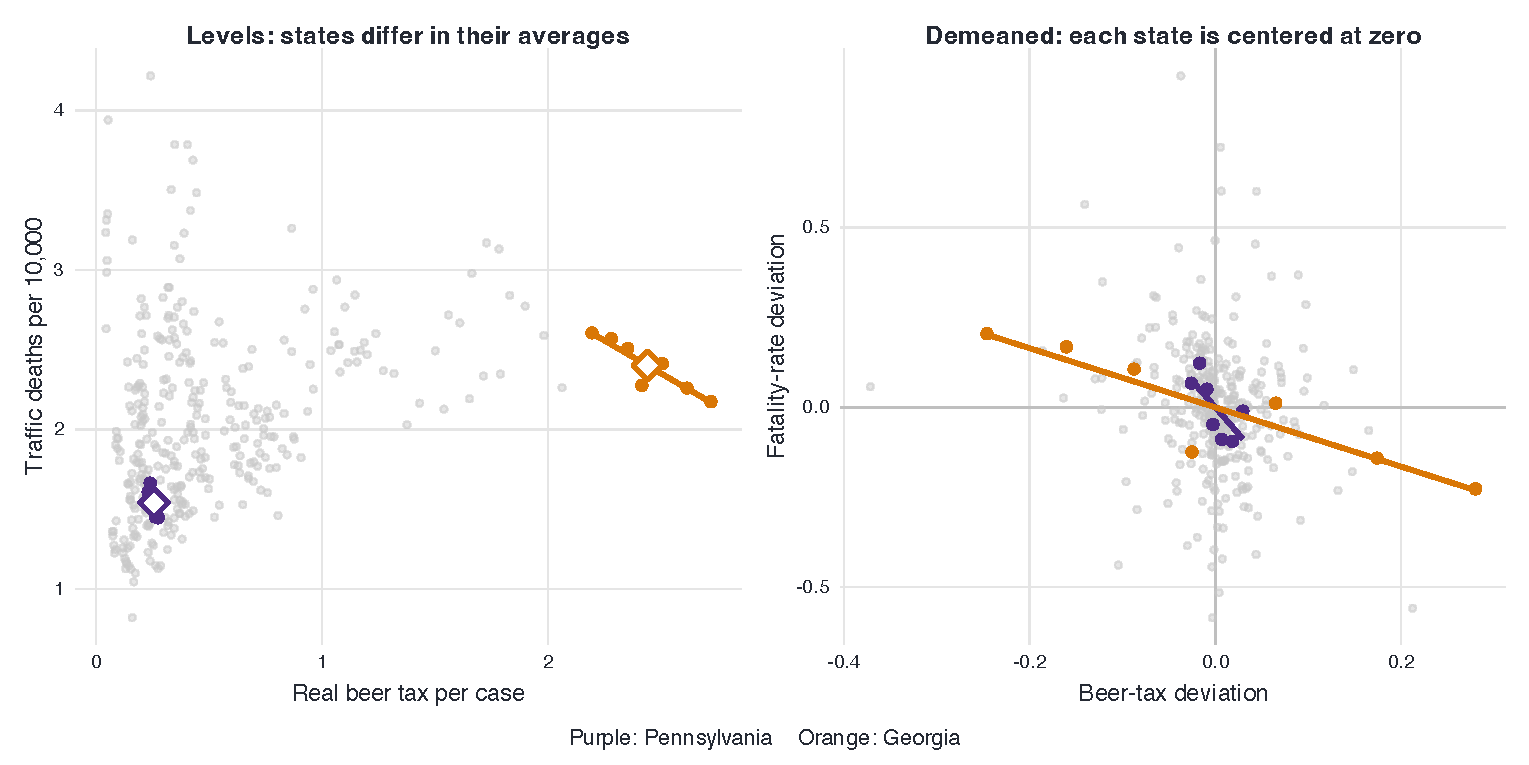
\includegraphics[height=0.62\textheight]{within_between_two_states_2026.pdf}
\end{center}
\vspace{-0.4em}
\begin{itemize}\itemsep0.25em
\item<2-> Colored dots are annual observations; colored lines are state-specific fits.
\item<2-> Gray dots show all other state-years; diamonds show state means.
\item<3-> The right panel subtracts each state's mean on both axes.
\end{itemize}
\slidesource{U.S. traffic-fatality panel; \textcite{ruhm1996alcohol} and \textcite{stock2007introduction}.}
\end{frame}


\begin{frame}
  \frametitle{Fixed Effects Regression}
  \small
\begin{itemize}
\item Our unobserved effects model is:
\[
y_{it} = \x_{it}\b + c_i + \varepsilon_{it}, \quad \quad t=1,2,...,T
\]\vspace{-.2in}
\item If we have data on multiple time periods, we can think of $c_i$ as \alert{fixed effects} or ``nuisance parameters'' to be estimated\bigskip\pause
\item OLS estimation with fixed effects yields:
\[
(\widehat{\b}, \widehat c_1,\ldots,\widehat c_N) = \underset{\bs{b},m_1,...,m_N}{\operatorname{argmin}}
\sum_{i=1}^N \sum_{t=1}^T (y_{it}-\x_{it}\bs{b}-m_i)^2
\]
this amounts to including $N$ farm dummies in regression of $y_{it}$ on $\x_{it}$
\end{itemize}
\end{frame}


\begin{frame}
  \frametitle{Derivation: Fixed Effects Regression}
  \small
%OLS estimation with fixed effects yields
\[
(\widehat \b, \widehat c_1,\ldots,\widehat c_N) = \underset{\bs{b},m_1,...,m_N}{\operatorname{argmin}}
\sum_{i=1}^N \sum_{t=1}^T (y_{it}-\x_{it}\bs{b}-m_i)^2
\]\\\bigskip
The first-order conditions (FOC) for this minimization problem are:
\[
\sum_{i=1}^N \sum_{t=1}^T \x_{it}'(y_{it}-\x_{it}\widehat\b-\widehat c_i)=0
\]
and
\[
\sum_{t=1}^T (y_{it}-\x_{it}\widehat\b-\widehat c_i)=0
\]
for $i=1,\ldots,N$.
\end{frame}

\begin{frame}
  \frametitle{Derivation: Fixed Effects Regression}
  \small
Therefore, for $i=1,\ldots,N$,
\[
\widehat c_i= \frac{1}{T} \sum_{t=1}^T (y_{it} -
\x_{it}\widehat\b) = \bar y_i-\bar \x_i\widehat\b,
\]
where
\[\bar \x_i \equiv \frac{1}{T} \sum_{t=1}^T \x_{it},\qquad
\bar y_i \equiv \frac{1}{T} \sum_{t=1}^T y_{it}.\]\pause

Plug this result into the first FOC to obtain:
\[
\widehat\b\! =\! \left(\sum_{i=1}^N \sum_{t=1}^T
(\x_{it}-\bar \x_i)' (\x_{it}-\bar \x_i) \right)^{-1}\!\!
\left( \sum_{i=1}^N
\sum_{t=1}^T (\x_{it}-\bar \x_i)'(y_{it}-\bar y_i)\right)
\]
\[
\widehat\b\! =\! \left(\sum_{i=1}^N \sum_{t=1}^T
\ddot{\x}_{it}' \ddot{\x}_{it} \right)^{-1}\!\!
\left(\sum_{i=1}^N
\sum_{t=1}^T \ddot{\x}_{it}' \ddot{y}_{it}\right)
\]
with time-demeaned variables $\ddot{\x}_{it}\equiv\x_{it}-\bar \x_i, \ddot{y}_{it}\equiv y_{it}-\bar y_i$.
\end{frame}

\begin{frame}
  \frametitle{Fixed Effects Regression}
  \small
Running a regression with the time-demeaned variables
$\ddot{y}_{it}\equiv y_{it}-\bar y_i$ and $\ddot{\x}_{it}\equiv\x_{it}-\bar \x_i$ is
numerically equivalent to a regression of $y_{it}$ on $\x_{it}$ and unit specific dummy variables.\bigskip\pause

Fixed effects estimator is often called the \alert{within estimator} because it only uses the time variation within each cross-sectional unit.\bigskip\pause

The regression with the time-demeaned variables is consistent for $\b$ even when $Cov[\x_{it},c_i]\neq0$, because time-demeaning eliminates the unobserved effects:
\[
\begin{array}{rcl}
y_{it} &=& \x_{it}\b +c_i + \varepsilon_{it}\bigskip\\
\bar y_{i} &=& \bar \x_{i}\b +c_i + \bar\varepsilon_{i}\bigskip\\ \hline\\
(y_{it}-\bar y_i ) &=& (\x_{it}-\bar \x_i)\b + (c_i-c_i) + (\varepsilon_{it}-\bar\varepsilon_i)\bigskip \\
\ddot{y}_{it} &=& \ddot{\x}_{it}\b + \ddot \varepsilon_{it}
\end{array}
\]
\end{frame}

\begin{frame}
  \frametitle{Panel Connectedness: Municipalities and Years}
\begin{center}
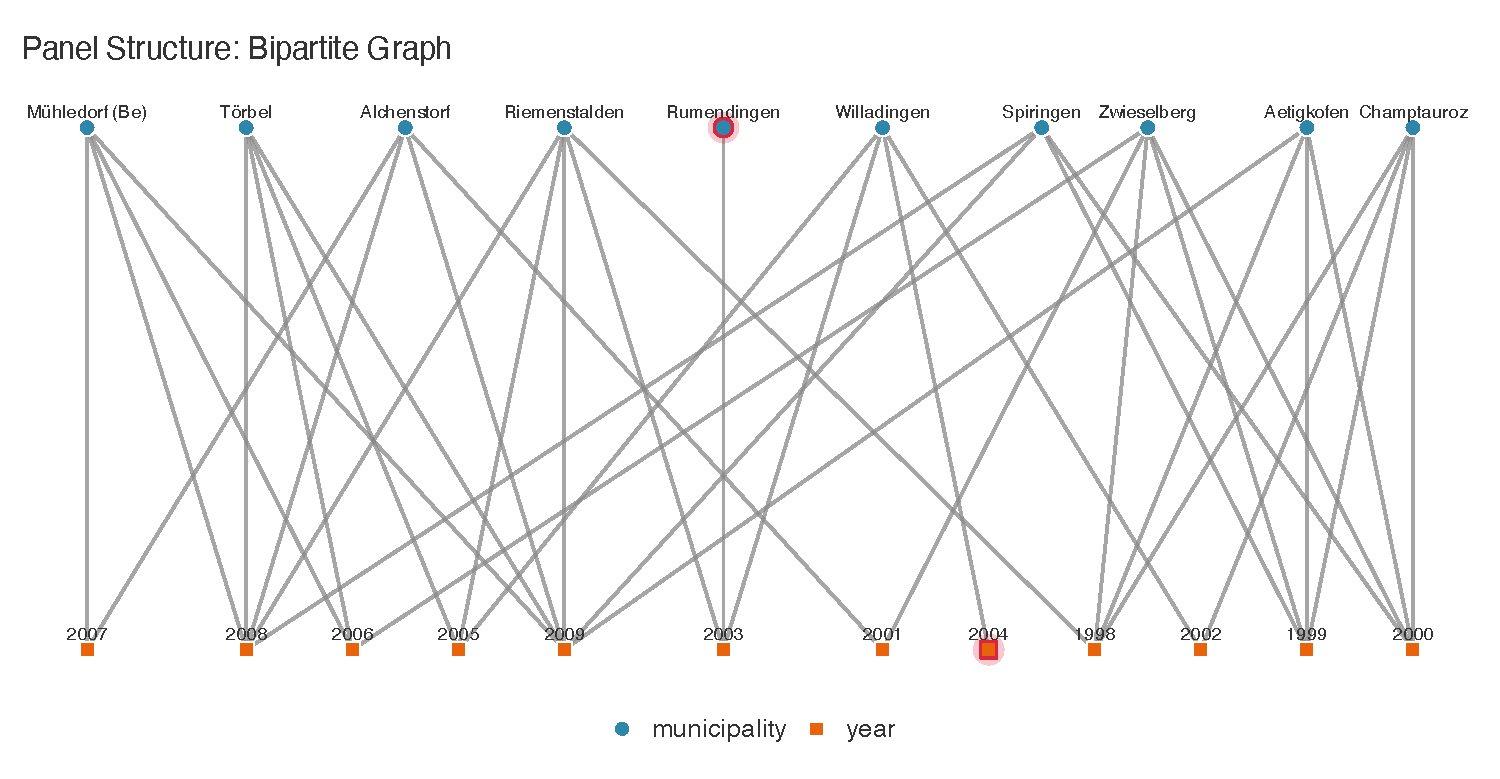
\includegraphics[height=0.61\textheight]{naturalization_network_2026.pdf}
\end{center}
\vspace{-0.6em}
\begin{itemize}\itemsep0.25em
\item<2-> A line marks a usable municipality--year observation.
\item<2-> Red rings mark a municipality or year represented once.
\item<3-> Rumendingen appears only in 2003, so it adds no within-municipality variation.
\end{itemize}
\slidesource{\textcite{hainmueller2019direct} replication data; selected municipalities, 1998--2009; \texttt{panelView(type = "network")}.}
\end{frame}


\if\solutions1
\begin{frame}
  \frametitle{Fixed Effects Regression: Main Results}
  \small
\begin{itemize}
  \item Identification assumptions:
  \begin{enumerate}
    \item $E[\varepsilon_{it}|\x_{i1},\x_{i2},...,\x_{iT},c_i]=0, \,\,t=1,2,...,T$
    \begin{itemize}
    \item regressors are \red{strictly exogenous conditional on the unobserved effect}
      \item allows $\x_{it}$ to be arbitrarily related to $c_i$
    \end{itemize}
    \item  $rank(\ddot{\X}) = K < NT$ and $E(\ddot{\x_i}?\ddot{\x_i})$ is p.d. and finite
           \begin{itemize}
      \item regressors vary over time for at least some $i$ and are not collinear
    \end{itemize}
  \end{enumerate}\pause
  \item Fixed effects estimator:
  \begin{enumerate}
    \item Demean and regress $\ddot{y}_{it}$ on $\ddot{\x}_{it}$ (need to correct degrees of freedom)
    \item Regress $y_{it}$ on $\x_{it}$ and unit dummies (dummy variable regression)
    \item Regress $y_{it}$ on $\x_{it}$ with canned fixed effects routine
    \begin{itemize}
      \item R: \texttt{fixest::feols(y \textasciitilde{} x | PanelID, data = d, cluster = \textasciitilde{} PanelID)}
    \end{itemize}
  \end{enumerate}\pause
   \item Properties (under assumptions 1-2):
  \begin{itemize}
    \item $\bhat_{FE}$ is consistent: $\underset{N\to\infty}{\operatorname{plim}}\,\bhat_{FE,N}  = \b$
    \item $\bhat_{FE}$ also unbiased conditional on $\X$
  \end{itemize}
\end{itemize}
\end{frame}
\fi


\if\solutions1
\begin{frame}
  \frametitle{Fixed Effects Regression: Main Issues}
  \small
\begin{itemize}[<+->]
  \item Inference:
  \begin{itemize}
    \item Standard errors have to be ``clustered'' by panel unit (e.g. farm) to allow correlation in the
$\varepsilon_{it}$'s for the same $i$.\medskip
\item Yields valid inference as long as number of clusters is reasonably large
\end{itemize}\bigskip
\item Typically we care about $\b$, but unit fixed effects $c_i$ could be of interest
    \begin{itemize}
     \item  $\widehat c_{i}$ from dummy variable regression is unbiased but not consistent for $c_i$ (based on fixed $T$ and $N \rightarrow \infty $)\medskip
     \item \red{\texttt{fixest::feols()}} absorbs the unit effects; recover their estimates with \red{\texttt{fixef()}}
\end{itemize}
\end{itemize}
\end{frame}
\fi


\begin{frame}
  \frametitle{Naturalization Panel: Variables and Timing}
\small
\begin{itemize}\itemsep0.8em
\item The panel contains 1,400 Swiss municipalities observed annually from 1991 to 2009.
\item The outcome is the naturalization rate:
\[
y_{it}=100\times
\frac{\text{naturalizations}_{it}}
{\text{eligible foreign population}_{i,t-1}}.
\]
\item $x_{it}=1$ when an elected municipal council decides applications and $0$ when citizens vote in referendums.
\item Some municipalities changed their decision rules over time.
\end{itemize}
\slidesource{\textcite{hainmueller2019direct}.}
\end{frame}


\if\solutions0
\begin{frame}[fragile]
  \frametitle{R Demo: Read and Inspect the Panel}
\begin{lstlisting}[language=R]
library(haven)
library(dplyr)
library(fixest)

d <- read_dta("figs/Swiss_Panel_long.dta") |>
  mutate(year = as.integer(year))

d |> select(muniID, muni_name, year,
            nat_rate, repdem) |> slice(30:38)
\end{lstlisting}
\begin{block}{Data structure}
4,655 municipality-years; 245 municipalities; 1991--2009.
\end{block}
\end{frame}
\fi

\if\solutions1
\begin{frame}
  \frametitle{Naturalization Panel Data}
\begin{center}
  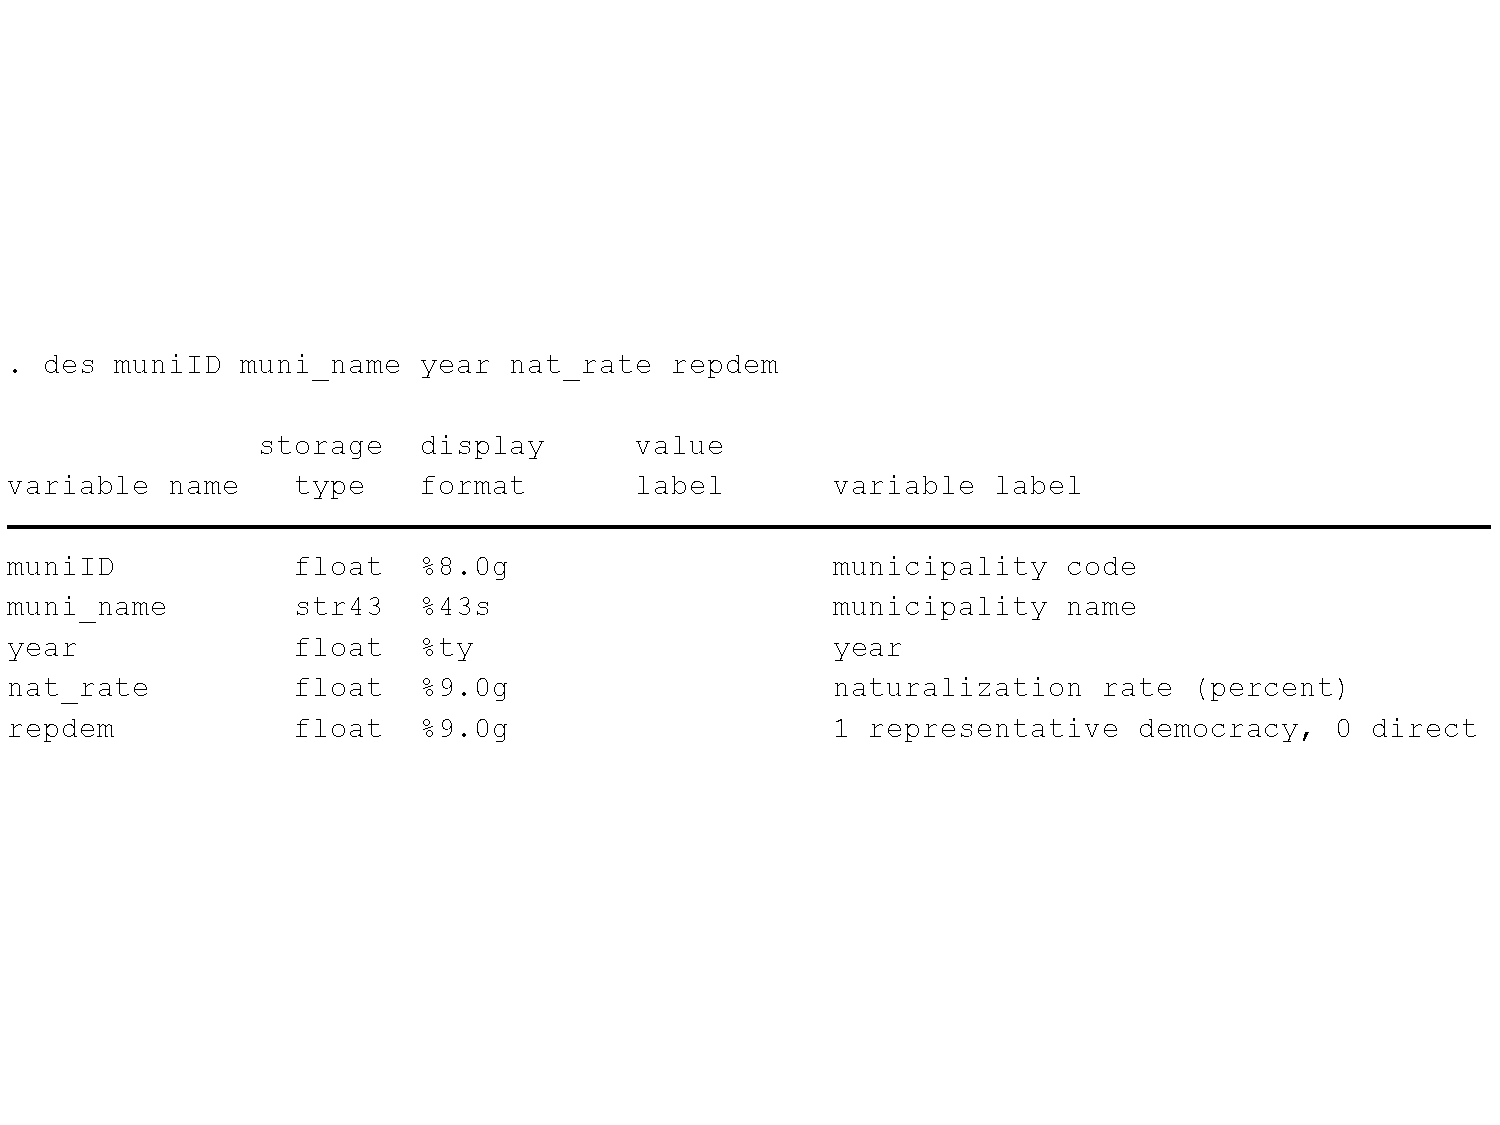
\includegraphics[height=1.5in,keepaspectratio=1]{S1.pdf}
\end{center}
\end{frame}
\fi

\if\solutions1
\begin{frame}
  \frametitle{Panel Data Long Format}
\begin{center}
  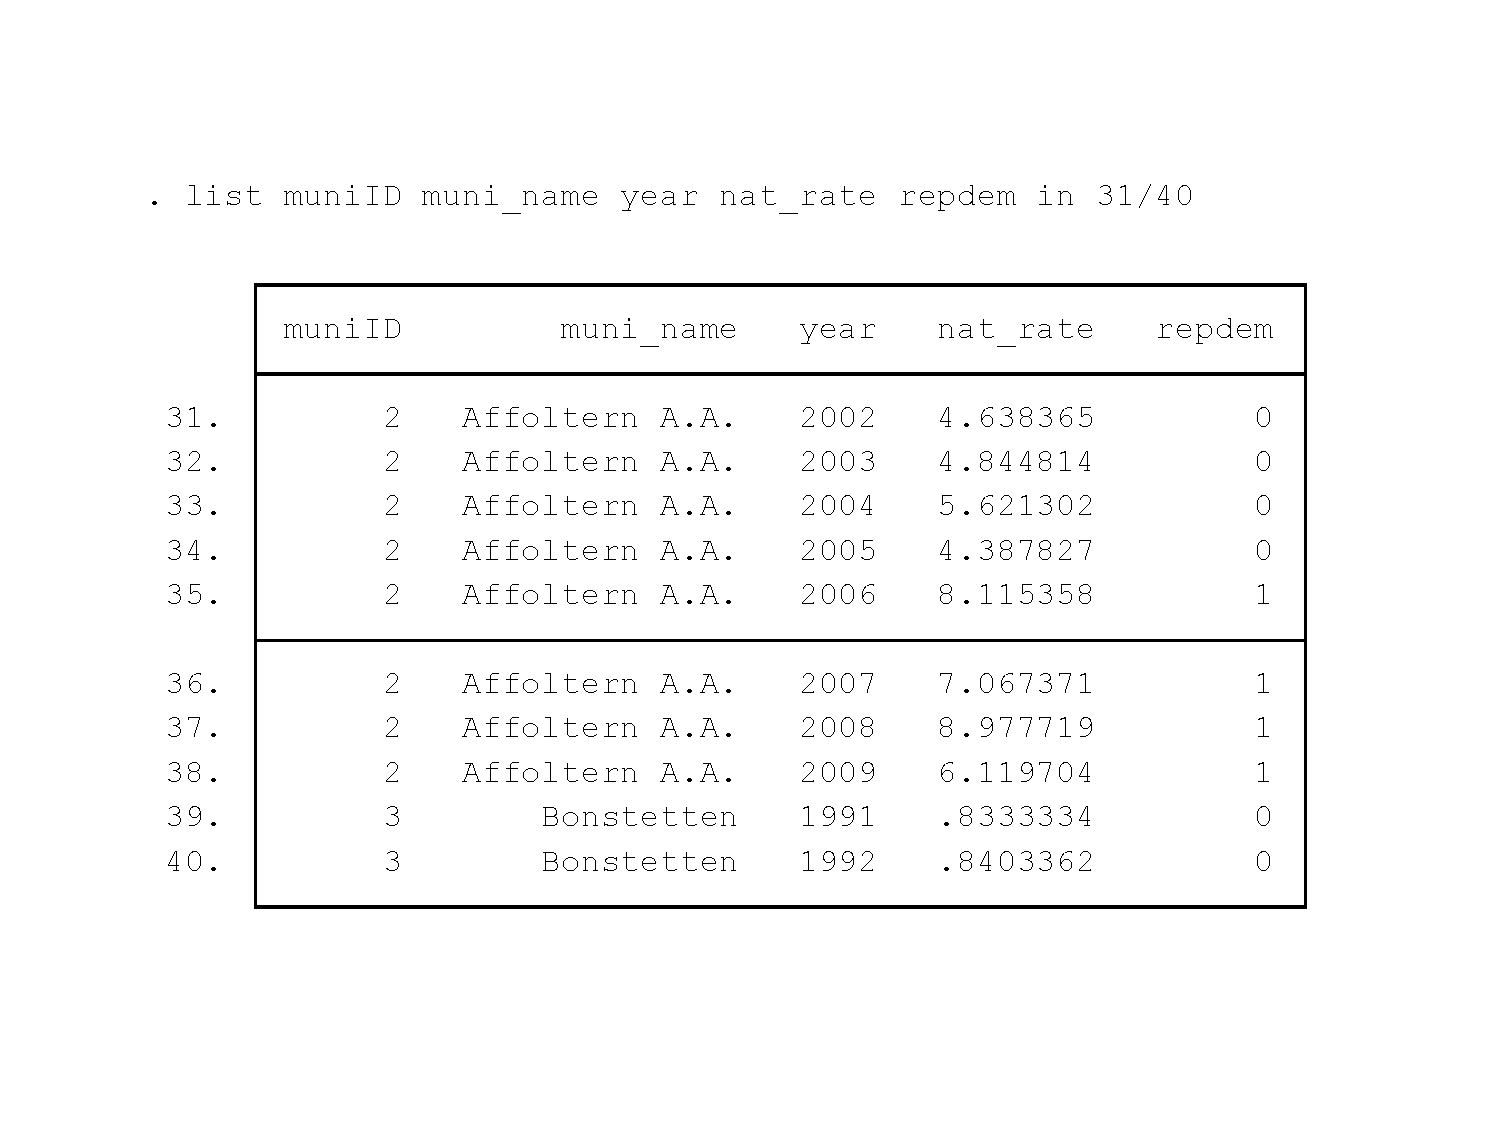
\includegraphics[height=2.9in,keepaspectratio=1]{S1a.pdf}
\end{center}
\end{frame}
\fi

\if\solutions1
\begin{frame}
  \frametitle{Pooled OLS}
\begin{center}\vspace{-.1in}
  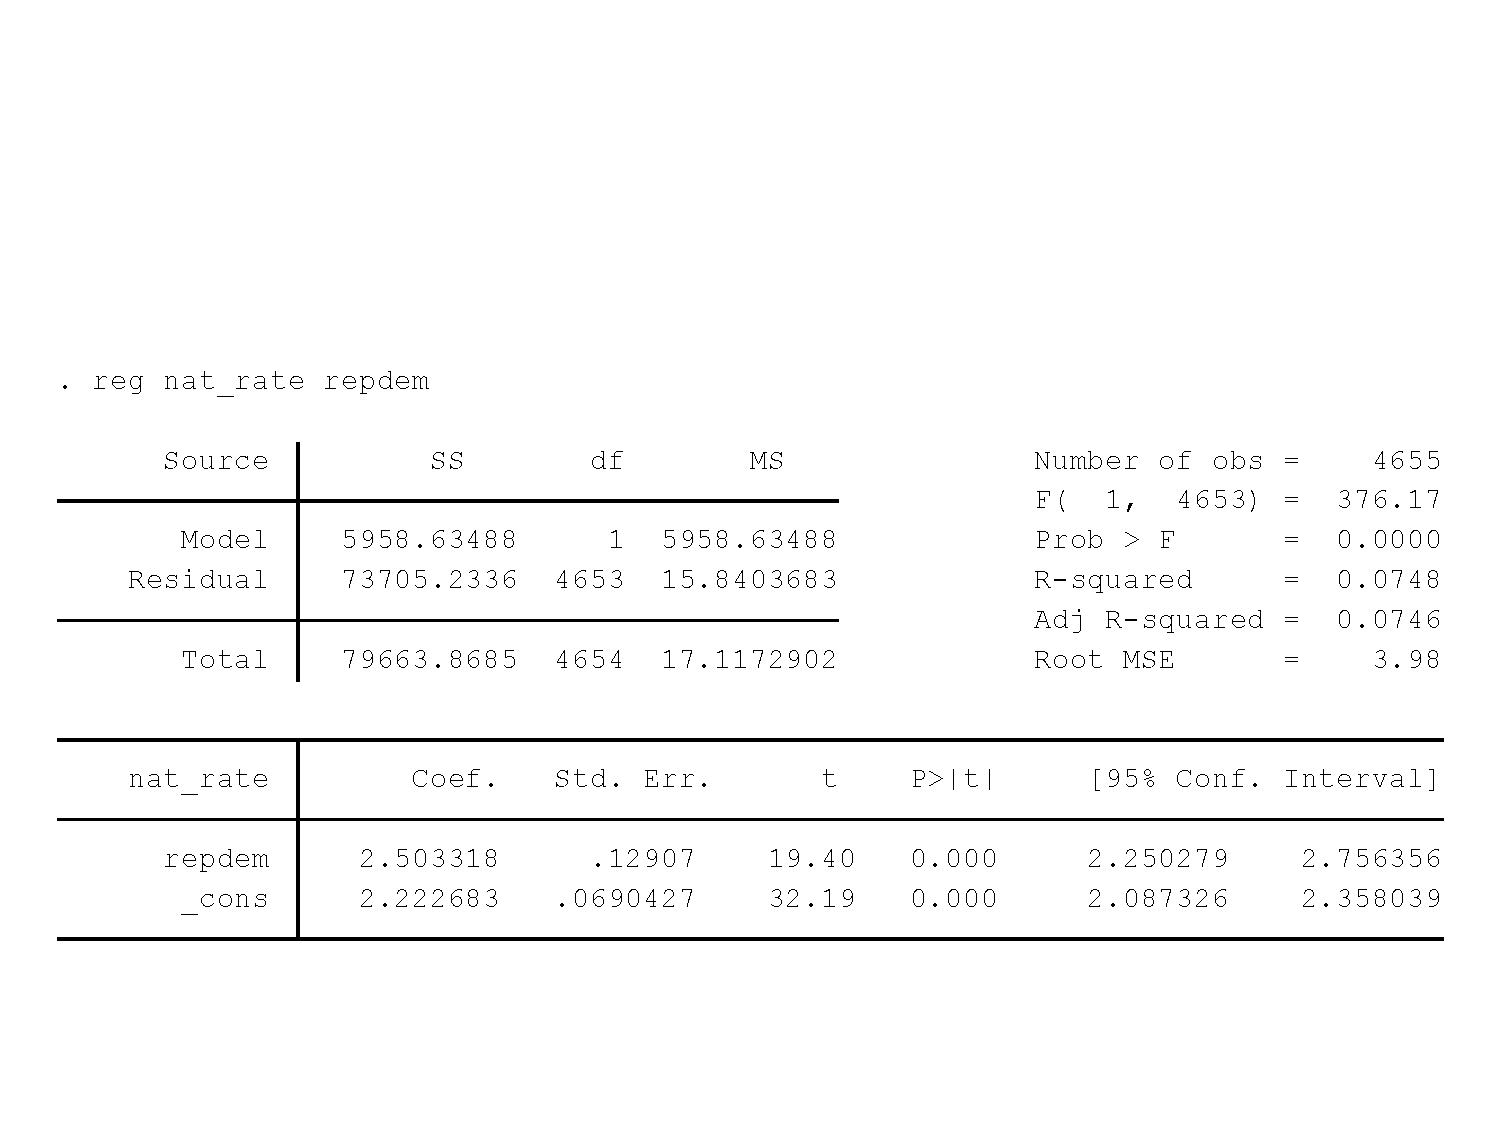
\includegraphics[height=2.1in,keepaspectratio=1]{POLS.pdf}
\end{center}
\end{frame}
\fi

\if\solutions0
\begin{frame}[fragile]
  \frametitle{R Demo: Pooled OLS}
\begin{lstlisting}[language=R]
m_pool <- feols(nat_rate ~ repdem, data = d)
etable(m_pool)
\end{lstlisting}
\begin{center}
\begin{tabular}{lrr}
 & Estimate & Standard error \\ \hline
Representative democracy & 2.503 & 0.129 \\
\end{tabular}
\end{center}
\keyquestion{Does the cross-sectional difference reflect a causal effect, or stable differences across municipalities?}
\end{frame}
\fi

\if\solutions1
\begin{frame}
  \frametitle{Decompose Within and Between Variation}
\begin{center}
  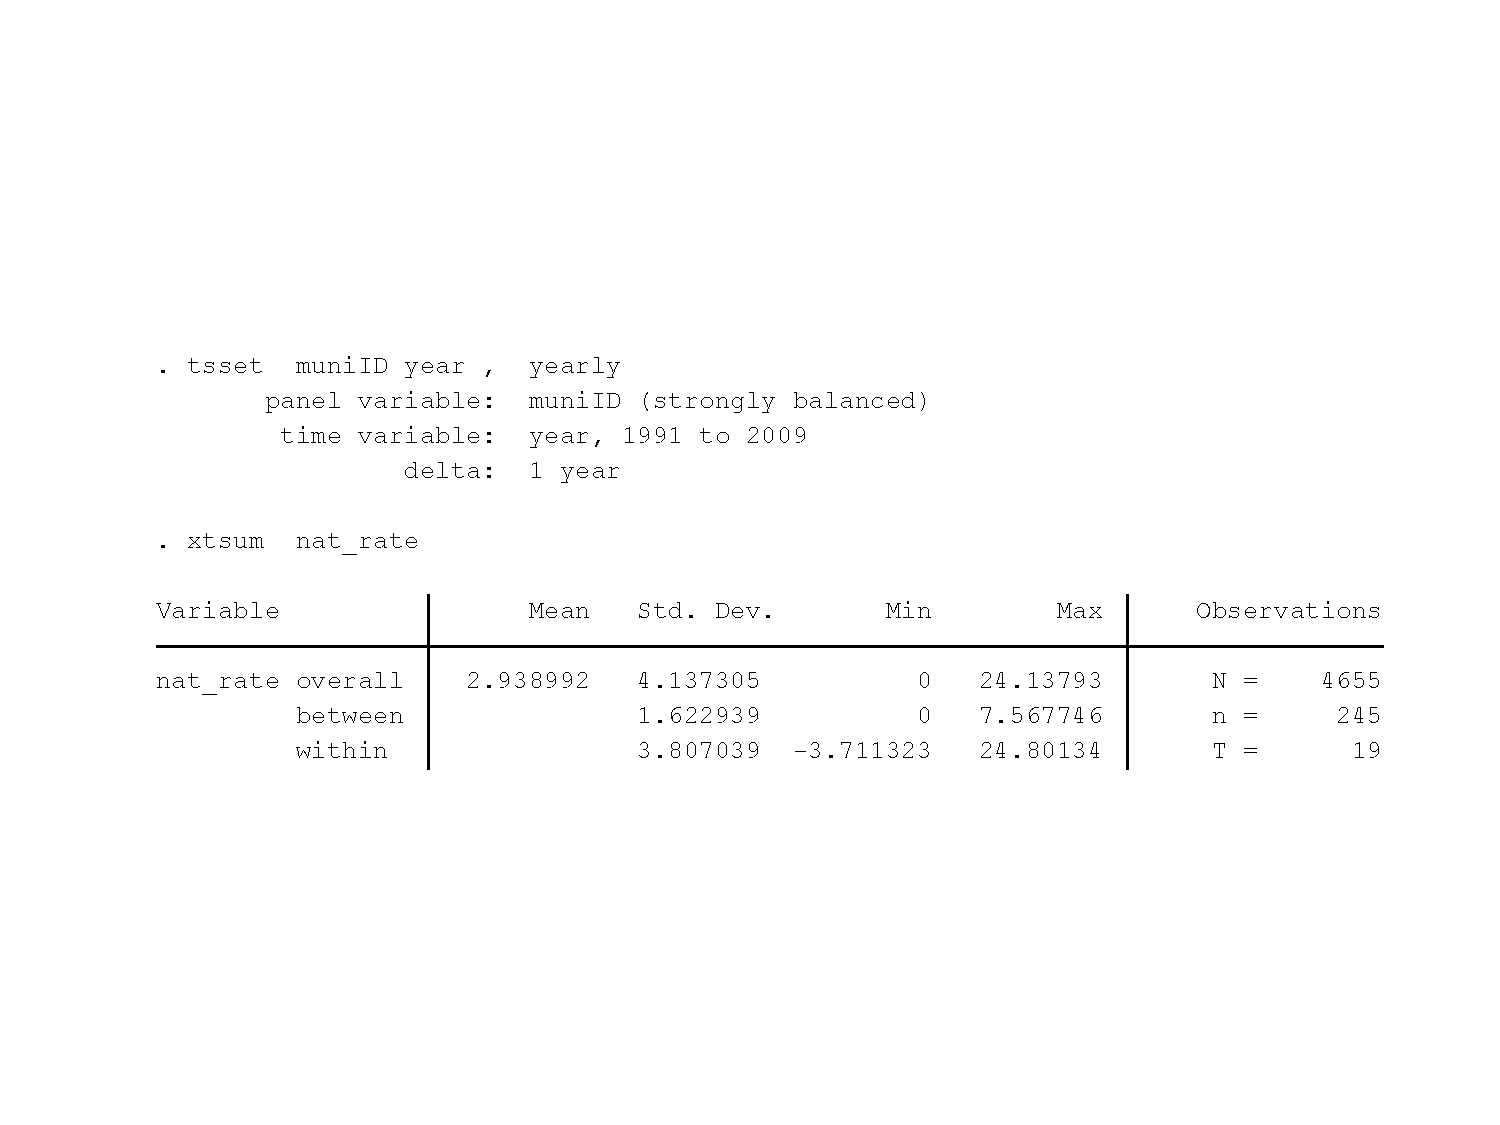
\includegraphics[height=1.8in,keepaspectratio=1]{S3.pdf}
\end{center}
\end{frame}
\fi

\if\solutions1
\begin{frame}
  \frametitle{Time-Demeaning for Fixed Effects: $y_{it}\rightarrow\ddot{y}_{it}$}
\begin{center}
  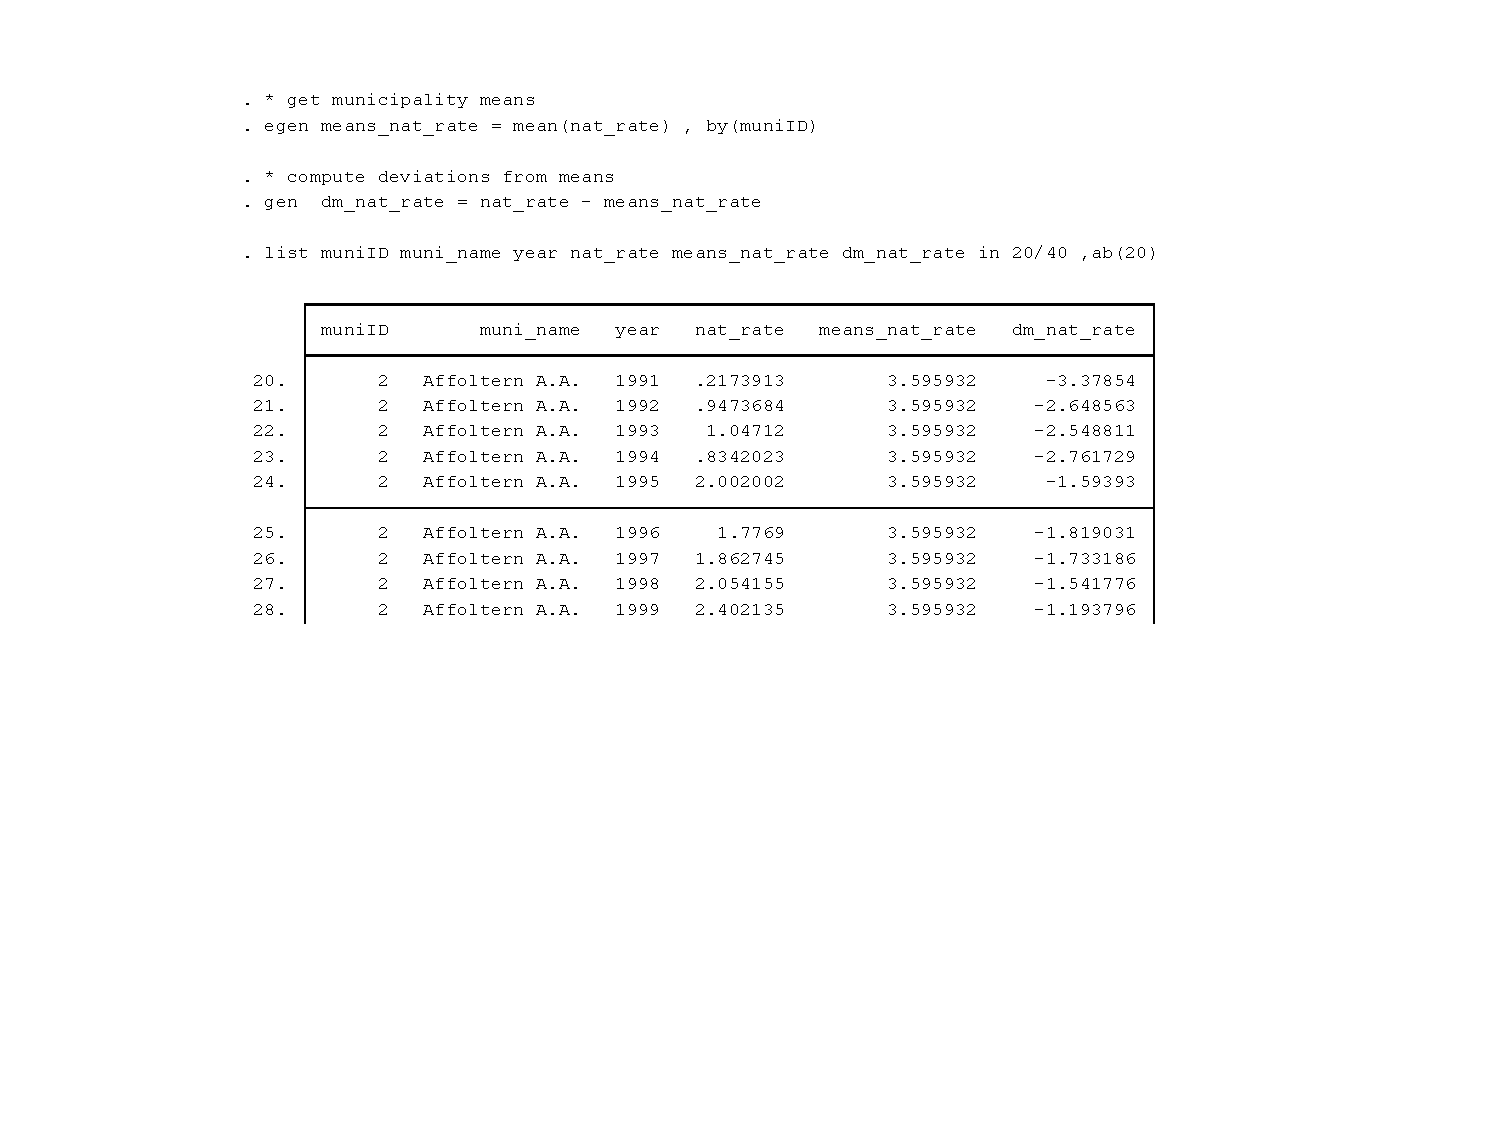
\includegraphics[height=2.7in,keepaspectratio=1]{S4.pdf}
\end{center}
\end{frame}
\fi

\if\solutions0
\begin{frame}[fragile]
  \frametitle{Time-Demeaning for Fixed Effects: $y_{it}\rightarrow\ddot{y}_{it}$}
\begin{lstlisting}[language=R]
d <- d |>
  group_by(muniID) |>
  mutate(across(c(nat_rate, repdem),
                ~ .x - mean(.x), .names = "{.col}_dm")) |>
  ungroup()

m_within <- feols(nat_rate_dm ~ repdem_dm, data = d)
\end{lstlisting}
\begin{block}{Within comparison}
The coefficient uses only changes within the same municipality.
\end{block}
\end{frame}
\fi

\if\solutions1
\begin{frame}
  \frametitle{Fixed Effects Regression with Demeaned Data}
\begin{center}\vspace{-.1in}
  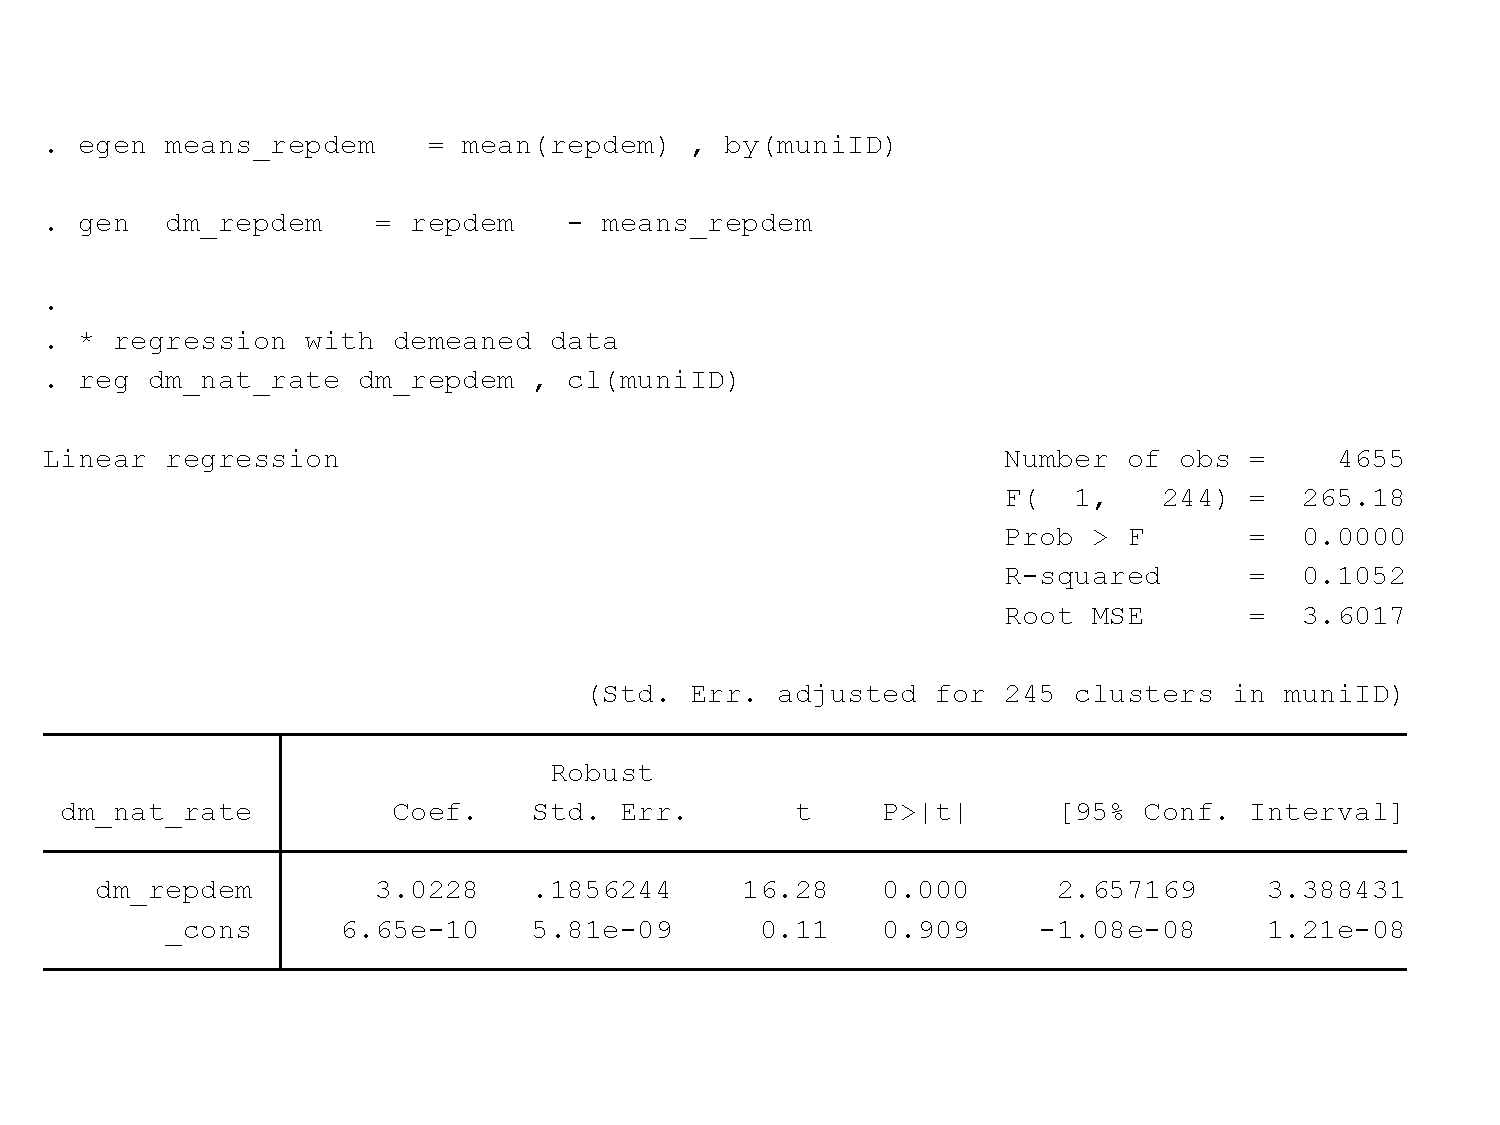
\includegraphics[height=2.9in,keepaspectratio=1]{S5.pdf}
\end{center}
\end{frame}
\fi

\if\solutions0
\begin{frame}[fragile]
  \frametitle{R Demo: Unit Fixed Effects}
\begin{lstlisting}[language=R]
m_fe <- feols(nat_rate ~ repdem | muniID,
              data = d, cluster = ~muniID)
\end{lstlisting}
\begin{center}
\begin{tabular}{lrr}
 & Estimate & Clustered SE \\ \hline
Representative democracy & 3.023 & 0.186 \\
\end{tabular}
\end{center}
\begin{itemize}
\item \texttt{| muniID} absorbs municipality fixed effects.
\item \texttt{cluster = ~muniID} allows serial correlation within municipalities.
\end{itemize}
\end{frame}
\fi

\if\solutions1
\begin{frame}
  \frametitle{Fixed Effects Regression with Canned Routine}
\begin{center}
  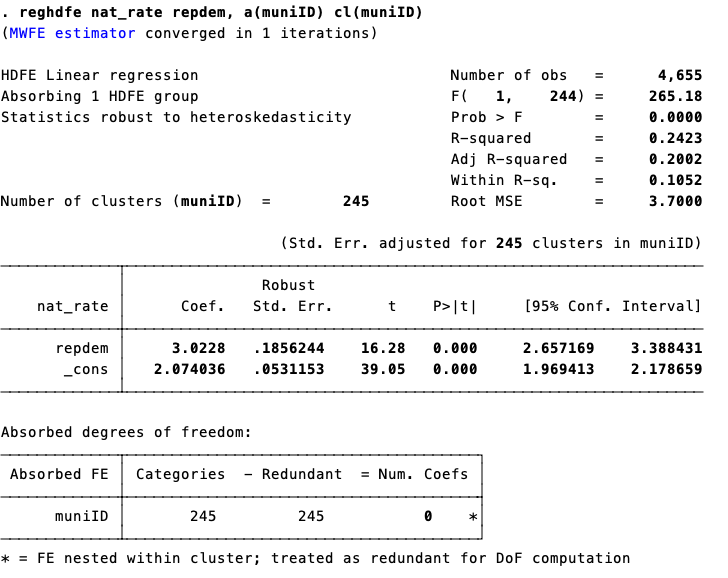
\includegraphics[height=2.8in,keepaspectratio=1]{S5b.png}
\end{center}
\end{frame}
\fi

\if\solutions0
\begin{frame}[fragile]
  \frametitle{R Demo: Add Year Fixed Effects}
\begin{lstlisting}[language=R]
m_twfe <- feols(nat_rate ~ repdem | muniID + year,
                data = d, cluster = ~muniID)
etable(m_fe, m_twfe)
\end{lstlisting}
\begin{center}
\begin{tabular}{lrr}
 & Unit FE & Unit + year FE \\ \hline
Representative democracy & 3.023 & 1.204 \\
Clustered SE & 0.186 & 0.303 \\
\end{tabular}
\end{center}
The coefficient falls sharply once year fixed effects remove changes common to all municipalities.
\end{frame}
\fi

\if\solutions1
\begin{frame}
  \frametitle{Fixed Effects Regression with Dummies}
\begin{center}
  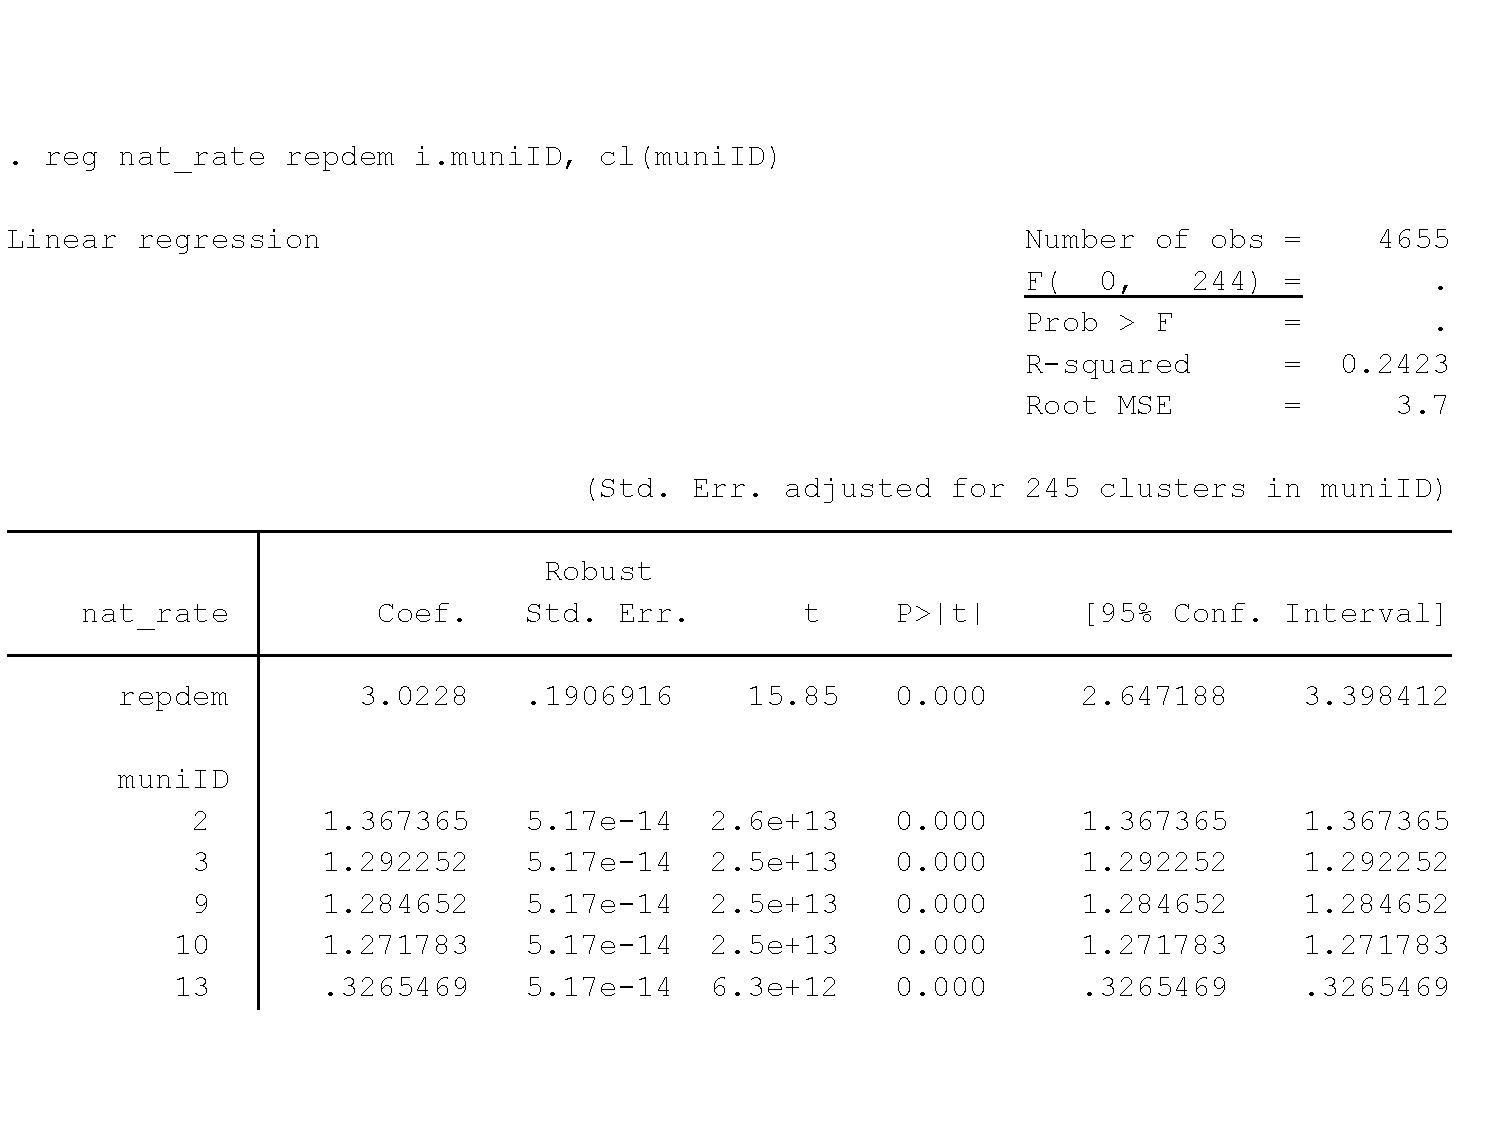
\includegraphics[height=2.9in,keepaspectratio=1]{S6.pdf}
\end{center}
\end{frame}
\fi

\if\solutions0
\begin{frame}[fragile]
  \frametitle{R Demo: Three Equivalent Ways to Fit Unit FE}
\begin{lstlisting}[language=R]
feols(nat_rate_dm ~ repdem_dm, data = d)
feols(nat_rate ~ repdem + i(muniID), data = d)
feols(nat_rate ~ repdem | muniID, data = d)
\end{lstlisting}
\begin{block}{Same coefficient, different computation}
Demeaning makes the within-municipality comparison explicit. For large panels, absorbing fixed effects is more convenient.
\end{block}
\end{frame}
\fi

\begin{frame}
  \frametitle{Random Effects}
\small
\[
y_{it}-\lambda\bar y_i
=
(\x_{it}-\lambda\bar\x_i)\b
+(v_{it}-\lambda\bar v_i),
\qquad 0\leq\lambda\leq1
\]
\begin{itemize}\itemsep0.7em
\item The random-effects estimator uses changes within units and differences in average levels across units.
\item The parameter $\lambda$ determines how much of each unit mean is subtracted.
\item It requires $E[c_i\mid\x_i]=0$: persistent unobserved unit differences are unrelated to all regressors.
\item It can estimate coefficients on time-invariant regressors.
\end{itemize}
\end{frame}

\begin{frame}
  \frametitle{Pooled OLS, Fixed Effects, and Random Effects}
\small
\begin{center}
\renewcommand{\arraystretch}{1.35}
\begin{tabular}{>{\raggedright\arraybackslash}p{0.25\textwidth}>{\raggedright\arraybackslash}p{0.33\textwidth}>{\raggedright\arraybackslash}p{0.33\textwidth}}
 & \textbf{Pooled OLS and random effects} & \textbf{Fixed effects} \\ \hline
Comparisons used & Within and between & Within each unit \\
Relation between $c_i$ and $\x_i$ & Assume no correlation & Allows correlation \\
Time-invariant regressors & Estimated & Not separately identified \\
Main risk & Time-invariant and time-varying confounding & Time-varying confounding; $x_{it}$ responds to earlier outcome shocks \\
\end{tabular}
\end{center}
\bigskip\pause
\begin{block}{Model choice}
Use fixed effects when stable unit differences may be correlated with the regressors. The random-effects model requires the design to make $E[c_i\mid\x_i]=0$ credible. Comparing the fixed- and random-effects estimates does not establish this assumption.
\end{block}
\end{frame}

\begin{frame}[fragile]
  \frametitle{R Demo: Beer Taxes and Traffic Fatalities}
\begin{lstlisting}[language=R,basicstyle=\ttfamily\footnotesize]
library(plm)
data("Fatalities", package = "AER")
Fatalities$fatal_rate <- with(Fatalities, fatal / pop * 10000)
p <- pdata.frame(Fatalities, index = c("state", "year"))

pool <- plm(fatal_rate ~ beertax, p, model = "pooling")
fe   <- plm(fatal_rate ~ beertax, p, model = "within")
re   <- plm(fatal_rate ~ beertax, p, model = "random")
twfe <- plm(fatal_rate ~ beertax, p,
            model = "within", effect = "twoways")

state_se <- function(m) sqrt(diag(vcovHC(
  m, method = "arellano", type = "HC1", cluster = "group")))
\end{lstlisting}
\begin{block}{Data}
The four models use 336 observations from 48 states over seven years.
\end{block}
\end{frame}

\begin{frame}
  \frametitle{Beer-Tax Results Across Models}
\begin{center}
\renewcommand{\arraystretch}{1.25}
\begin{tabular}{lc}
\textbf{Model} & \textbf{Beer-tax coefficient} \\ \hline
Pooled OLS & 0.365 (0.119) \\
Random effects & -0.052 (0.109) \\
State FE & -0.656 (0.289) \\
State + year FE & -0.640 (0.350) \\
\end{tabular}

\end{center}
\bigskip
\begin{itemize}\itemsep0.5em
\item<2-> Parentheses contain standard errors clustered by state using \texttt{state\_se()}.
\item<3-> Pooled OLS and state fixed effects give estimates with opposite signs.
\item<3-> The random-effects estimate lies between the pooled and state fixed-effects estimates.
\item<4-> A causal interpretation requires beer-tax changes to be unrelated to unobserved fatality shocks in every year.
\end{itemize}
\slidesource{Author's calculations using \texttt{AER::Fatalities}; \textcite{ruhm1996alcohol}; \textcite{stock2007introduction}.}
\end{frame}


\begin{frame}
  \frametitle{Problems that Fixed Effects Do Not Solve}
  \small
\[
y_{it} = \x_{it}\b + c_i + \varepsilon_{it}, \quad \quad t=1,2,...,T
\]\vspace{-.2in}
\begin{itemize}
  \item $y_{it}$ is murder rate and $x_{it}$ is police spending per capita\medskip
  \item What happens when we regress $y$ on $x$ and city fixed effects?\pause
\begin{itemize}
  \item $\bhat_{FE}$ inconsistent unless \red{strict exogeneity} conditional on $c_i$ holds
      \begin{itemize}
      \item $E[\varepsilon_{it}|\x_{i1},\x_{i2},...,\x_{iT},c_i]=0, \,\,t=1,2,...,T$
  \item implies $\varepsilon_{it}$ uncorrelated with past, current, and future regressors
\end{itemize}
\end{itemize}\pause
  \item Most common violations:
  \begin{enumerate}
    \item \alert{Time-varying omitted variables}
    \begin{itemize}
      \item economic boom leads to more police spending and fewer murders
      \item can include time-varying controls, but avoid post-treatment bias
    \end{itemize}\pause
    \item \alert{Simultaneity \& feedback}
    \begin{itemize}
     \item if city adjusts police based on past murder rate, then spending$_{t+1}$ is correlated with $\varepsilon_{t}$ (since higher $\varepsilon_{t}$ leads to higher murder rate at $t$)
     \item strictly exogenous $x$ cannot react to what happens to $y$ in the past or the future!
\end{itemize}
  \end{enumerate}\pause
\item Fixed effects do not obviate need for good research design...
\end{itemize}
\end{frame}


% \end{frame}


% t test of coefficients:


\begin{frame}
  \frametitle{Summary: Fixed Effects, Pooled OLS (and Random Effects)}
\small
\begin{itemize}
\item[]
\begin{enumerate}
  \item[Assm. 1] Regressors are strictly exogenous conditional on the time-invariant unobservables
  \item[Assm. 2] Regressors are uncorrelated with time-varying \& time-invariant unobservables
\end{enumerate}\bigskip\pause
\item Results:
\begin{itemize}
\item Fixed effects estimator is consistent given Assm. 1, but rules out time-invariant regressors
\item Pooled OLS (and random effects) are consistent under Assum. 2, and allow for time-invariant regressors
\item Specification tests cannot establish a credible research design.
%\item Given homoscedasticity assumptions (random effects assumption 4), the random effects estimator is asymptotically efficient
\end{itemize}\bigskip\pause
\item Assum. 2 is strong, so fixed effects models are typically more credible
\begin{itemize}
  \item One main advantage of  panel data is to account for \red{time-invariant unobserved confounding}
\end{itemize}
\end{itemize}
\end{frame}


% 	Hausman Test


\section{Modeling Time}


\begin{frame}
  \frametitle{Common Changes in the Swiss Panel}
\begin{center}
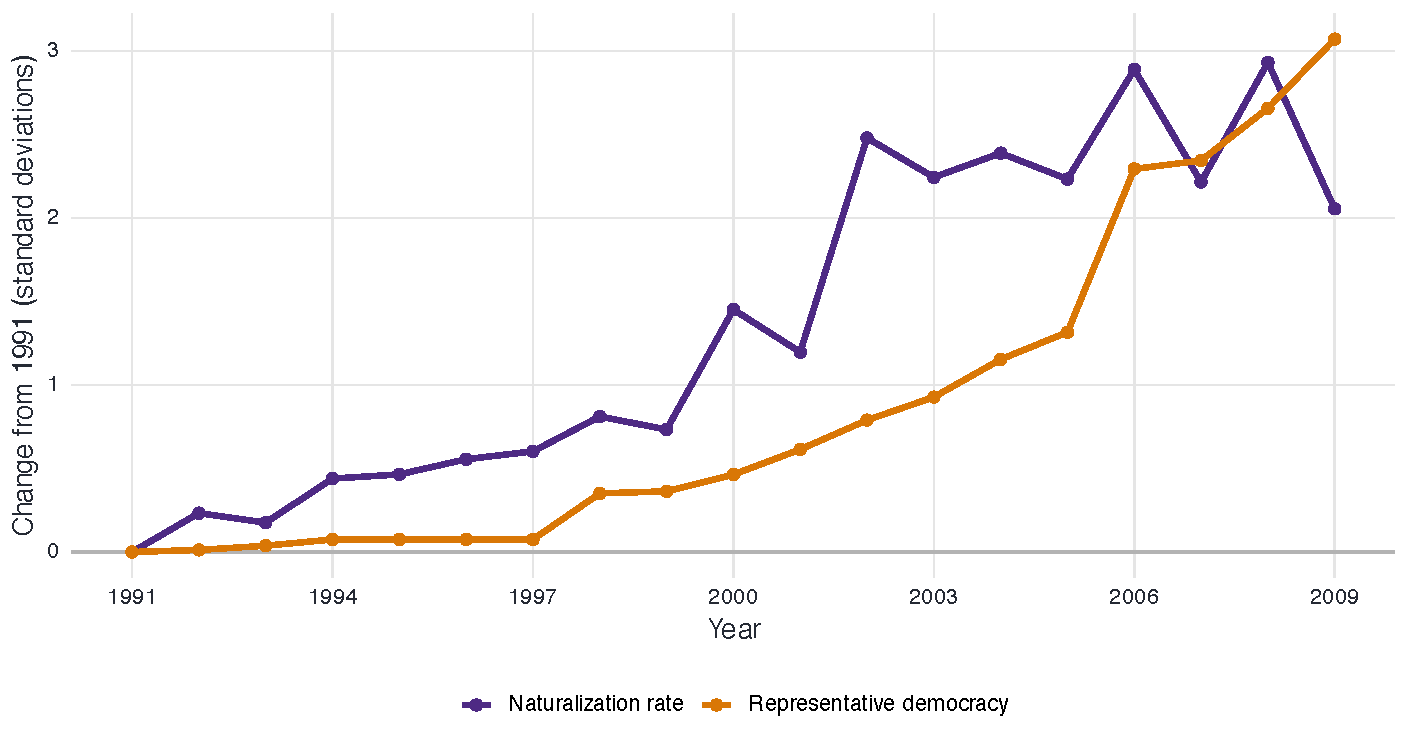
\includegraphics[height=0.68\textheight]{hh_common_shocks_2026.pdf}
\end{center}
\vspace{-0.5em}
\begin{itemize}\itemsep0.25em
\item From 1991 to 2009, both variables increase overall.
\item A nationwide change can be mistaken for the effect of a local institutional change.
\end{itemize}
\slidesource{\textcite{hainmueller2019direct}; author's calculations.}
\end{frame}

\begin{frame}
  \frametitle{Common Linear Trend}
\begin{columns}[T]
\column{.72\textwidth}
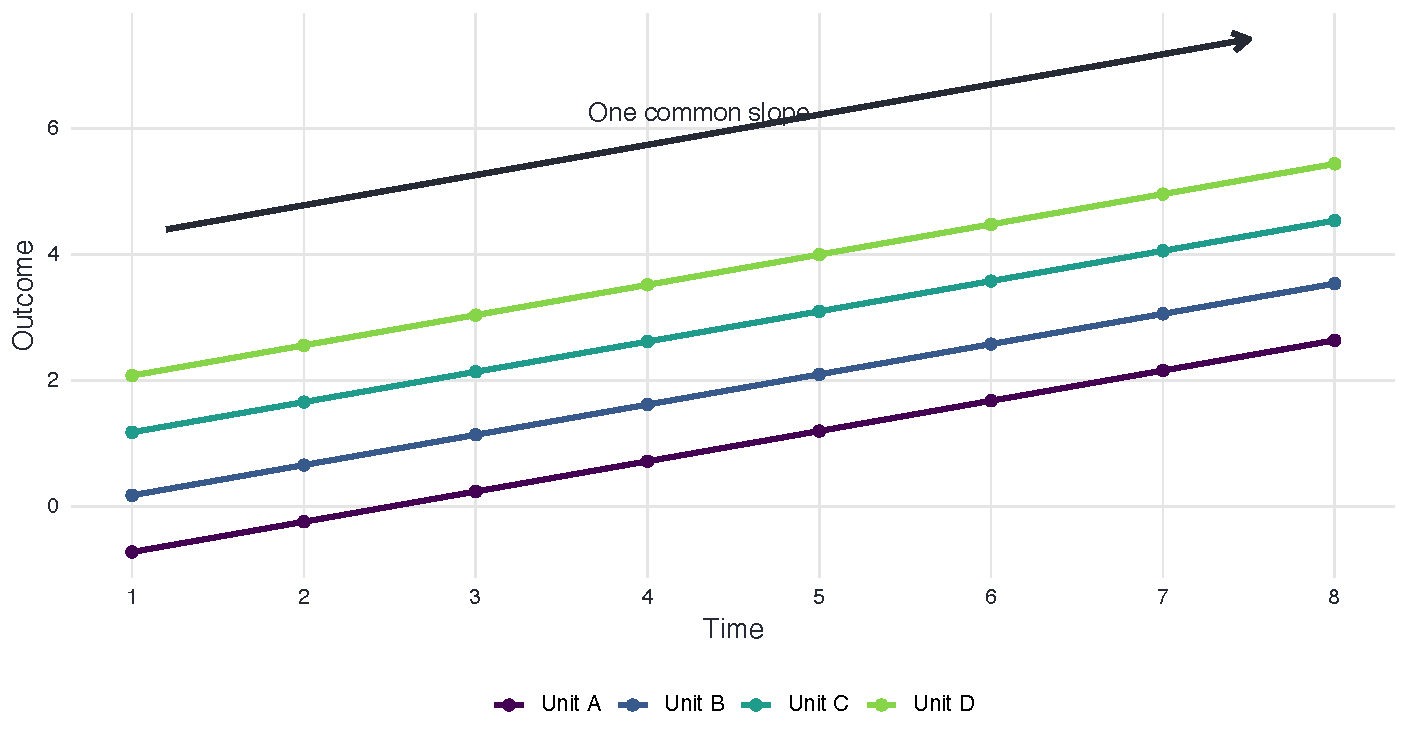
\includegraphics[width=\linewidth]{time_common_trend_2026.pdf}
\column{.27\textwidth}
\[
y_{it}=\x_{it}\b+c_i+\gamma t+\varepsilon_{it}
\]
\begin{block}{Common-trend assumption}
The model assumes the same linear time trend for every unit: $\gamma$ per period after accounting for $\x_{it}$ and $c_i$.
\end{block}
\end{columns}
\end{frame}

\begin{frame}
  \frametitle{Year Fixed Effects}
\begin{columns}[T]
\column{.72\textwidth}
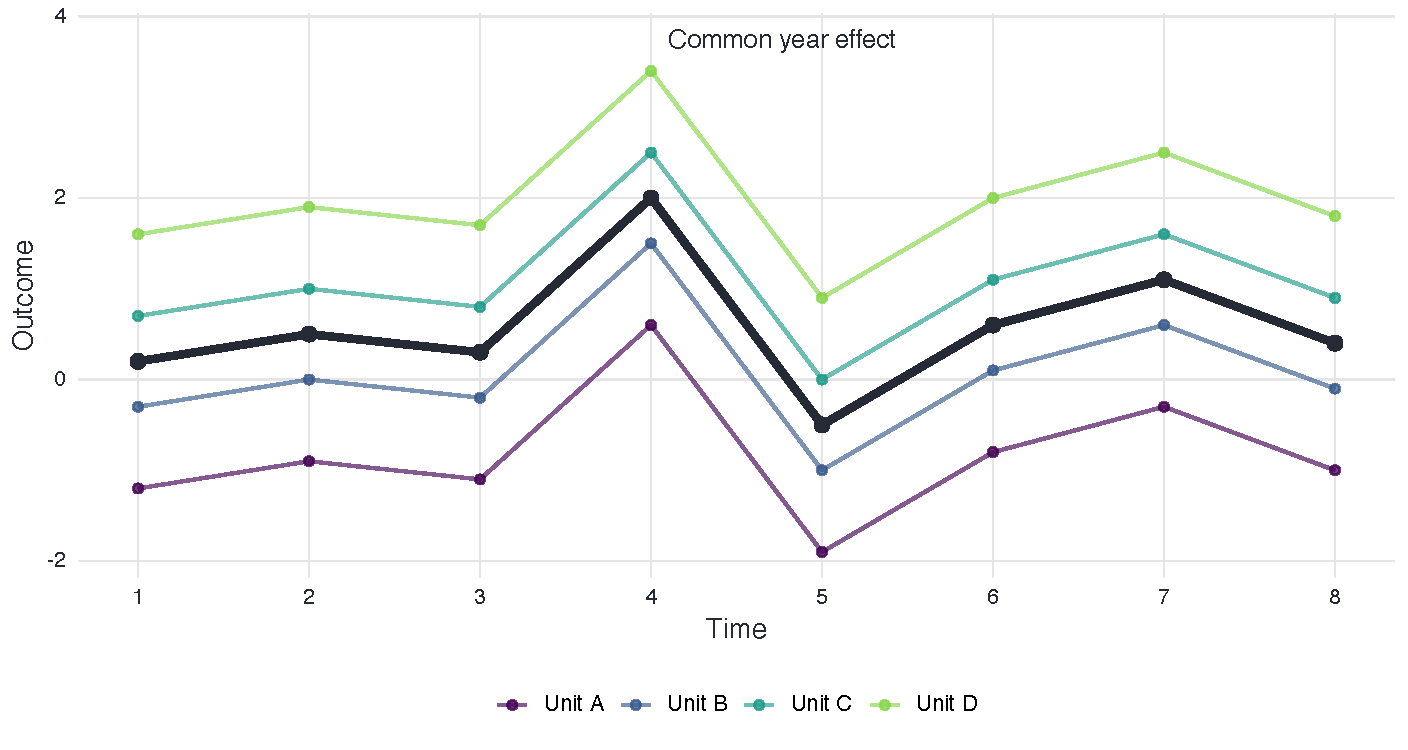
\includegraphics[width=\linewidth]{time_year_fe_2026.pdf}
\column{.27\textwidth}
\[
y_{it}=\x_{it}\b+c_i+\delta_t+\varepsilon_{it}
\]
\begin{block}{Year-effect assumption}
The model gives each year its own shift $\delta_t$ and assumes that shift is the same for every unit.
\end{block}
\end{columns}
\end{frame}

\begin{frame}
  \frametitle{Unit-Specific Linear Trends}
\begin{columns}[T]
\column{.72\textwidth}
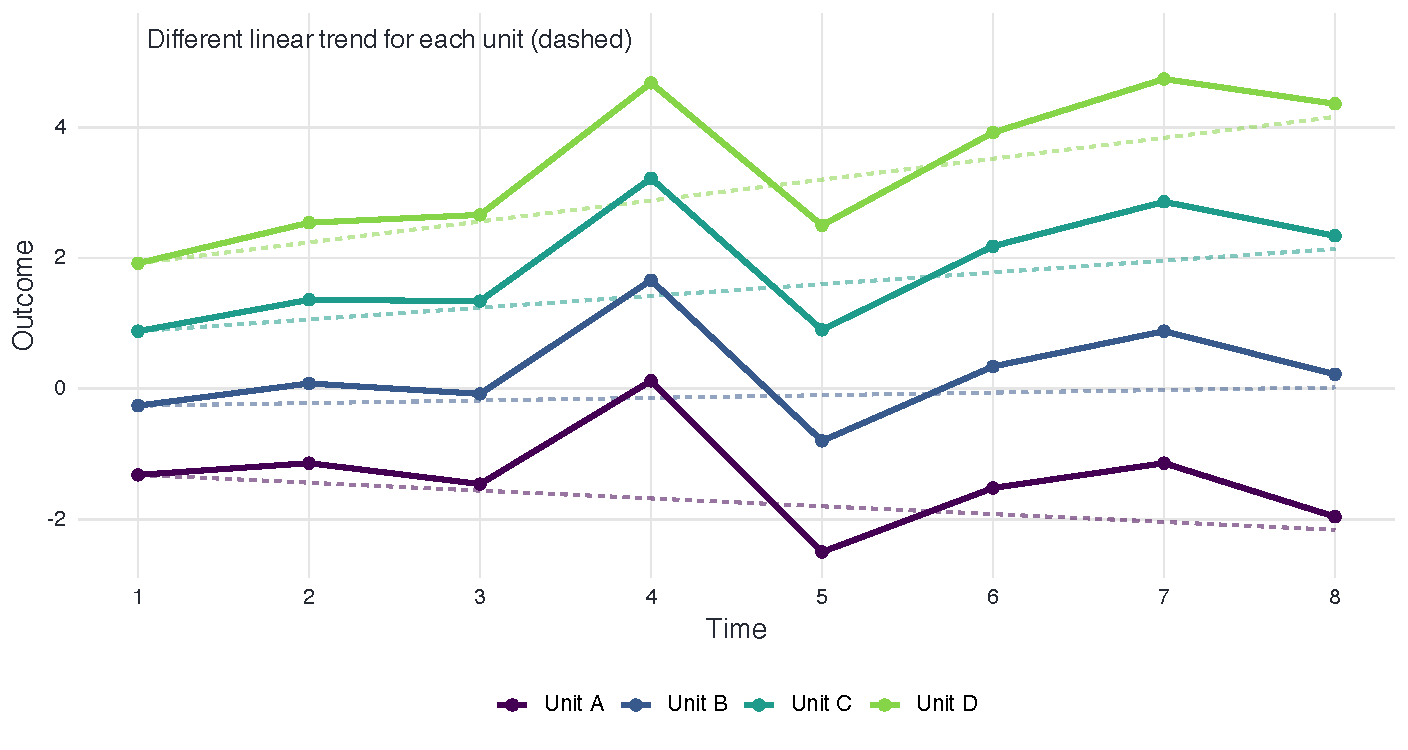
\includegraphics[width=\linewidth]{time_unit_trends_2026.pdf}
\column{.27\textwidth}
\[
y_{it}=\x_{it}\b+c_i+g_i t+\delta_t+\varepsilon_{it}
\]
\begin{block}{Unit-trend assumption}
After accounting for $\x_{it}$, $c_i$, and $\delta_t$, unit $i$ may follow its own linear trend $g_i t$.
\end{block}
\smallskip
\footnotesize After removing a separate linear trend for every unit, little within-unit treatment variation may remain.
\end{columns}
\end{frame}

\begin{frame}
  \frametitle{Naturalization Results Across Time Models}
\begin{center}
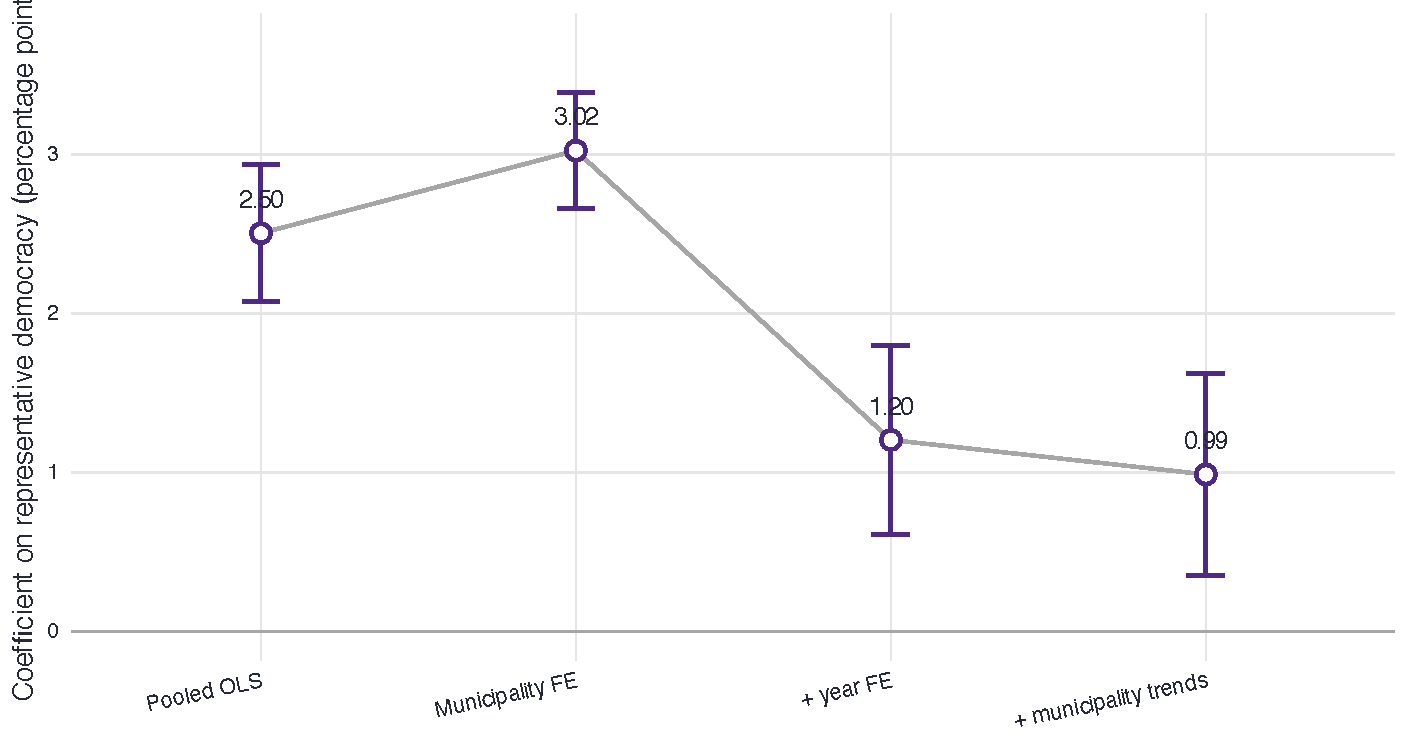
\includegraphics[height=0.64\textheight]{hh_time_controls_2026.pdf}
\end{center}
\vspace{-0.5em}
\begin{itemize}\itemsep0.25em
\item Year fixed effects remove changes shared across municipalities.
\item Municipality-specific trends remove each municipality's fitted linear change.
\end{itemize}
\slidesource{\textcite{hainmueller2019direct}; 95\% confidence intervals use municipality-clustered standard errors.}
\end{frame}


\if\solutions1
\begin{frame}
  \frametitle{Fixed Effects Regression: Linear Time Trend}
\begin{center}
  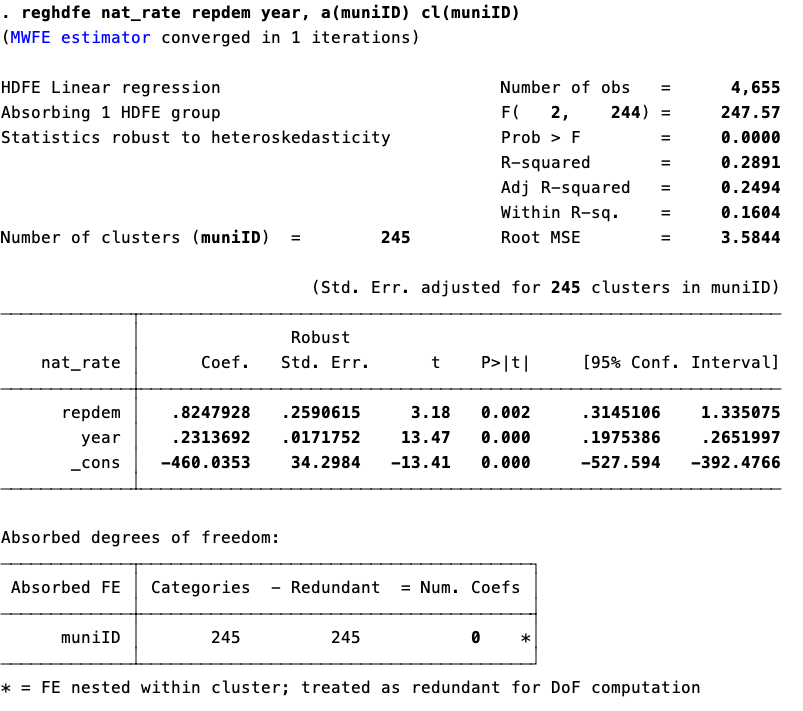
\includegraphics[height=3in,keepaspectratio=1]{T1a.png}
\end{center}
\end{frame}
\fi


% t test of coefficients:


\if\solutions1
\begin{frame}
  \frametitle{Fixed Effects Regression: Year Fixed Effects}
\begin{center}
  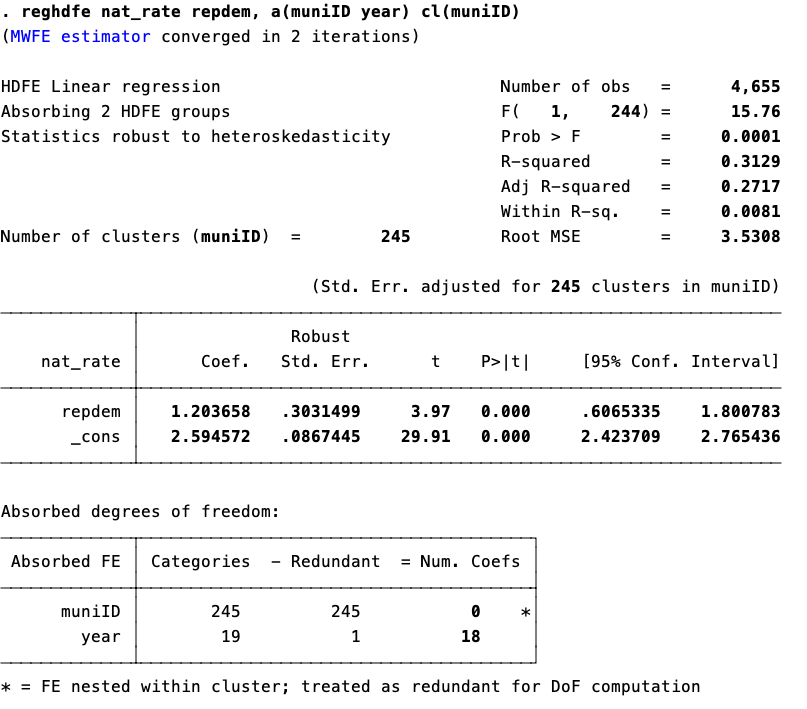
\includegraphics[height=3in,keepaspectratio=1]{T1aa.png}
\end{center}
\end{frame}
\fi


% t test of coefficients:

%          Estimate Std. Error t value  Pr(>|t|)    
% repdem    1.20366    0.30253  3.9786 7.043e-05 ***
% year1992  0.38292    0.17197  2.2266   0.02602 *  
% year1993  0.27898    0.15110  1.8463   0.06492 .  
% year1994  0.70341    0.16712  4.2089 2.617e-05 ***
% year1995  0.74591    0.17827  4.1841 2.919e-05 ***
% year1996  0.89693    0.18345  4.8892 1.049e-06 ***
% year1997  0.97570    0.18661  5.2285 1.788e-07 ***
% year1998  1.21550    0.22506  5.4007 6.988e-08 ***
% year1999  1.08051    0.21430  5.0419 4.794e-07 ***
% year2000  2.23993    0.23968  9.3457 < 2.2e-16 ***
% year2001  1.75531    0.24790  7.0807 1.662e-12 ***
% year2002  3.82573    0.32672 11.7096 < 2.2e-16 ***
% year2003  3.37837    0.32664 10.3428 < 2.2e-16 ***
% year2004  3.53176    0.34285 10.3012 < 2.2e-16 ***
% year2005  3.20837    0.31097 10.3171 < 2.2e-16 ***
% year2006  3.92057    0.39023 10.0468 < 2.2e-16 ***
% year2007  2.77646    0.36884  7.5276 6.237e-14 ***
% year2008  3.84780    0.40135  9.5872 < 2.2e-16 ***
% year2009  2.22388    0.41997  5.2953 1.246e-07 ***
% ---
% \end{verbatim}
% \end{frame}
% \fi


\if\solutions1
\begin{frame}
  \frametitle{Fixed Effects Regression: Unit Specific Time Trends}
\begin{center}\vspace{-.1in}
  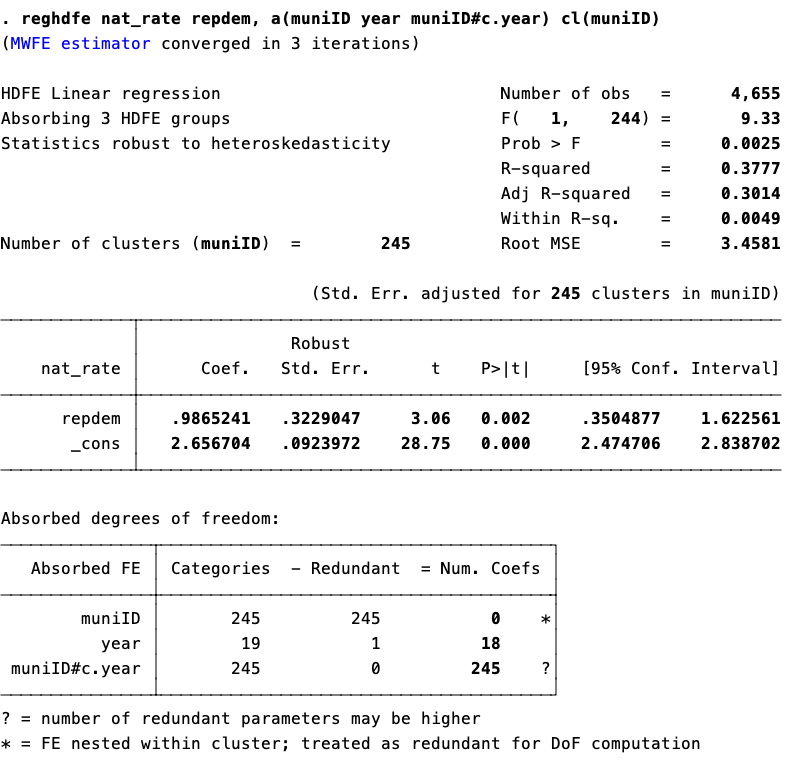
\includegraphics[height=3in,keepaspectratio=1]{T1aaa.png}
\end{center}
\end{frame}
\fi


% t test of coefficients:


\if\solutions1
\begin{frame}
  \frametitle{Unit Specific Quadratic Time Trends}
\begin{center}
  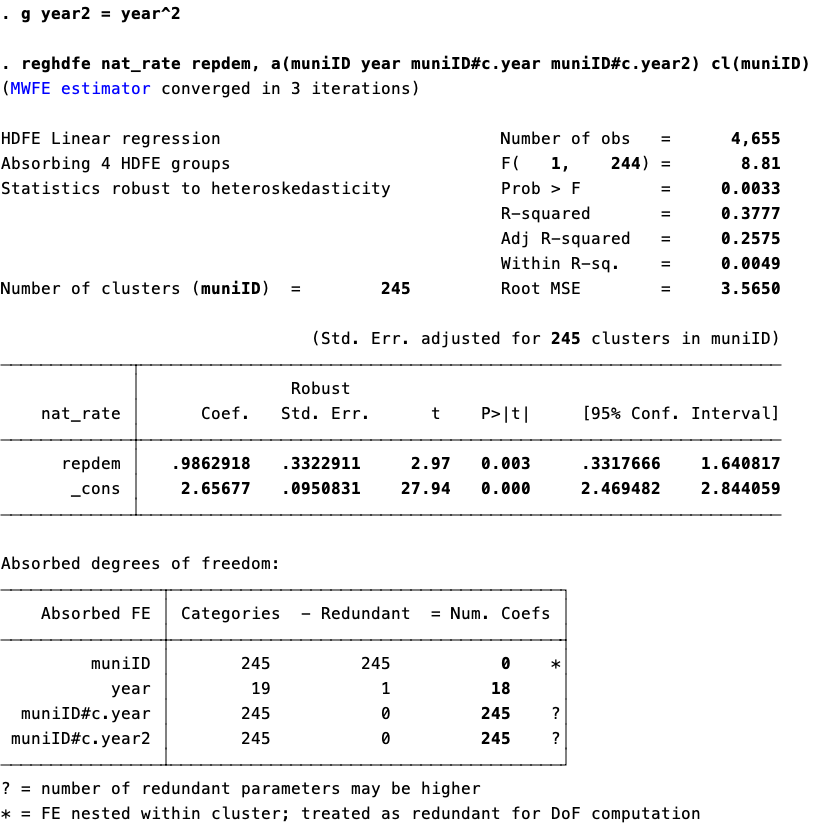
\includegraphics[height=3in,keepaspectratio=1]{T1aaaa.png}
\end{center}
\end{frame}
\fi


% t test of coefficients:


\section{Modeling Dynamic \& Heterogeneous Effects}


\begin{frame}
  \frametitle{Distributed Lag Model}
\vspace{-.2in}
\[
y_{it} =  x_{it}\b_0 + x_{it-1}\b_1 + x_{it-2}\b_2+ c_i + \varepsilon_{it}, \quad \quad t=1,2,...,T
\]\vspace{-.2in}
\begin{itemize}
   \item Model recognizes that effect of change in $x$ may occur with a lag
   \begin{itemize}
     \item effect of new tax credit for children on fertility rate
      \end{itemize}\medskip
    \item Interpretation of coefficients:\pause
      \begin{itemize}
      \item Consider \alert{temporary increase} in $x_{it}$ from level $m$ to $m+1$ at $t$, which lasts only one period
      \begin{itemize}
        \item[] $y_{t-1}= m \b_0 + m \b_1 + m \b_2+ c_i$
        \item[] $y_{t}\quad= \alert{(m+1)} \b_0 + m \b_1 + m \b_2+ c_i$
        \item[] $y_{t+1}= m \b_0 + \alert{(m+1)} \b_1 + m \b_2+ c_i$
        \item[] $y_{t+2}= m \b_0 + m \b_1 + \alert{(m+1)} \b_2+ c_i$
        \item[] $y_{t+3}= m \b_0 + m \b_1 + m \b_2+ c_i$
      \end{itemize}
      \end{itemize}
  \begin{itemize}[<+->]
    \item $\b_0=y_{t}-y_{t-1}$ immediate change in $y$ due to temporary one-unit increase in $x$ (impact propensity)
    \item $\b_1=y_{t+1}-y_{t-1}$ change in $y$ one period after temporary one-unit increase in $x$
    \item $\b_2=y_{t+2}-y_{t-1}$ change in $y$ two periods after temporary one-unit increase in $x$
    \item $y_{t+3}=y_{t-1}$ change in $y$ is zero three periods after temporary one-unit increase in $x$
  \end{itemize}
\end{itemize}
\end{frame}


\if\solutions1
\begin{frame}
  \frametitle{Lagged Effects of Direct Democracy}
\begin{center}
  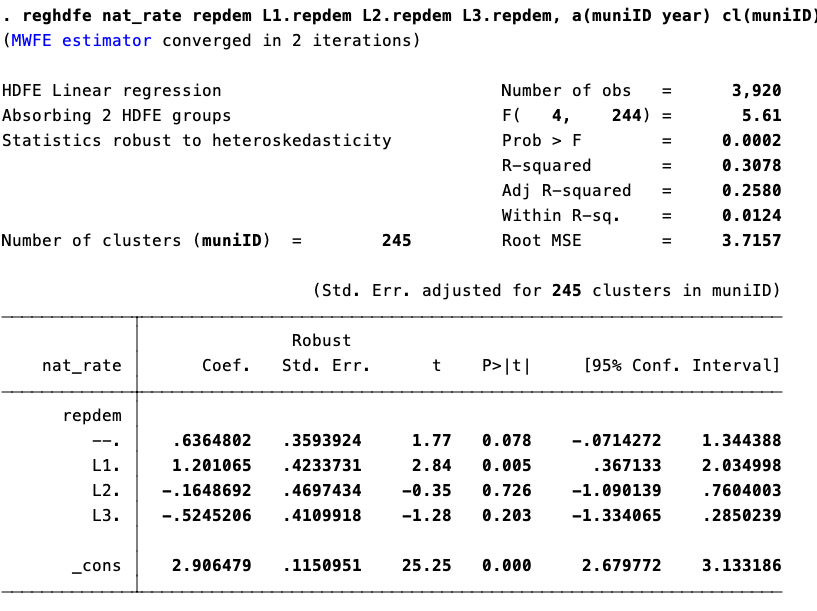
\includegraphics[height=2.9in,keepaspectratio=1]{FDL.png}
\end{center}
\end{frame}
\fi


% \small
% \begin{verbatim}
% > mod_lag    <- plm(nat_rate~repdem+
%   lag(repdem,1)+lag(repdem,2)+lag(repdem,3)+
% +                     year,data=d,model="within")
% > coeftest(mod_lag, vcov=function(x) 
% vcovHC(x, cluster="group", type="HC1"))
% t test of coefficients:
%                 Estimate Std. Error t value  Pr(>|t|)    
% repdem          0.636480   0.358658  1.7746  0.076044 .  
% lag(repdem, 1)  1.201065   0.422508  2.8427  0.004498 ** 
% lag(repdem, 2) -0.164869   0.468783 -0.3517  0.725087    
% lag(repdem, 3) -0.524521   0.410152 -1.2788  0.201033    
% year1995        0.031281   0.204172  0.1532  0.878244    
% year1996        0.188603   0.210878  0.8944  0.371183


\if\solutions1
\begin{frame}
  \frametitle{Long-run Effect of Direct Democracy}
\begin{center}
  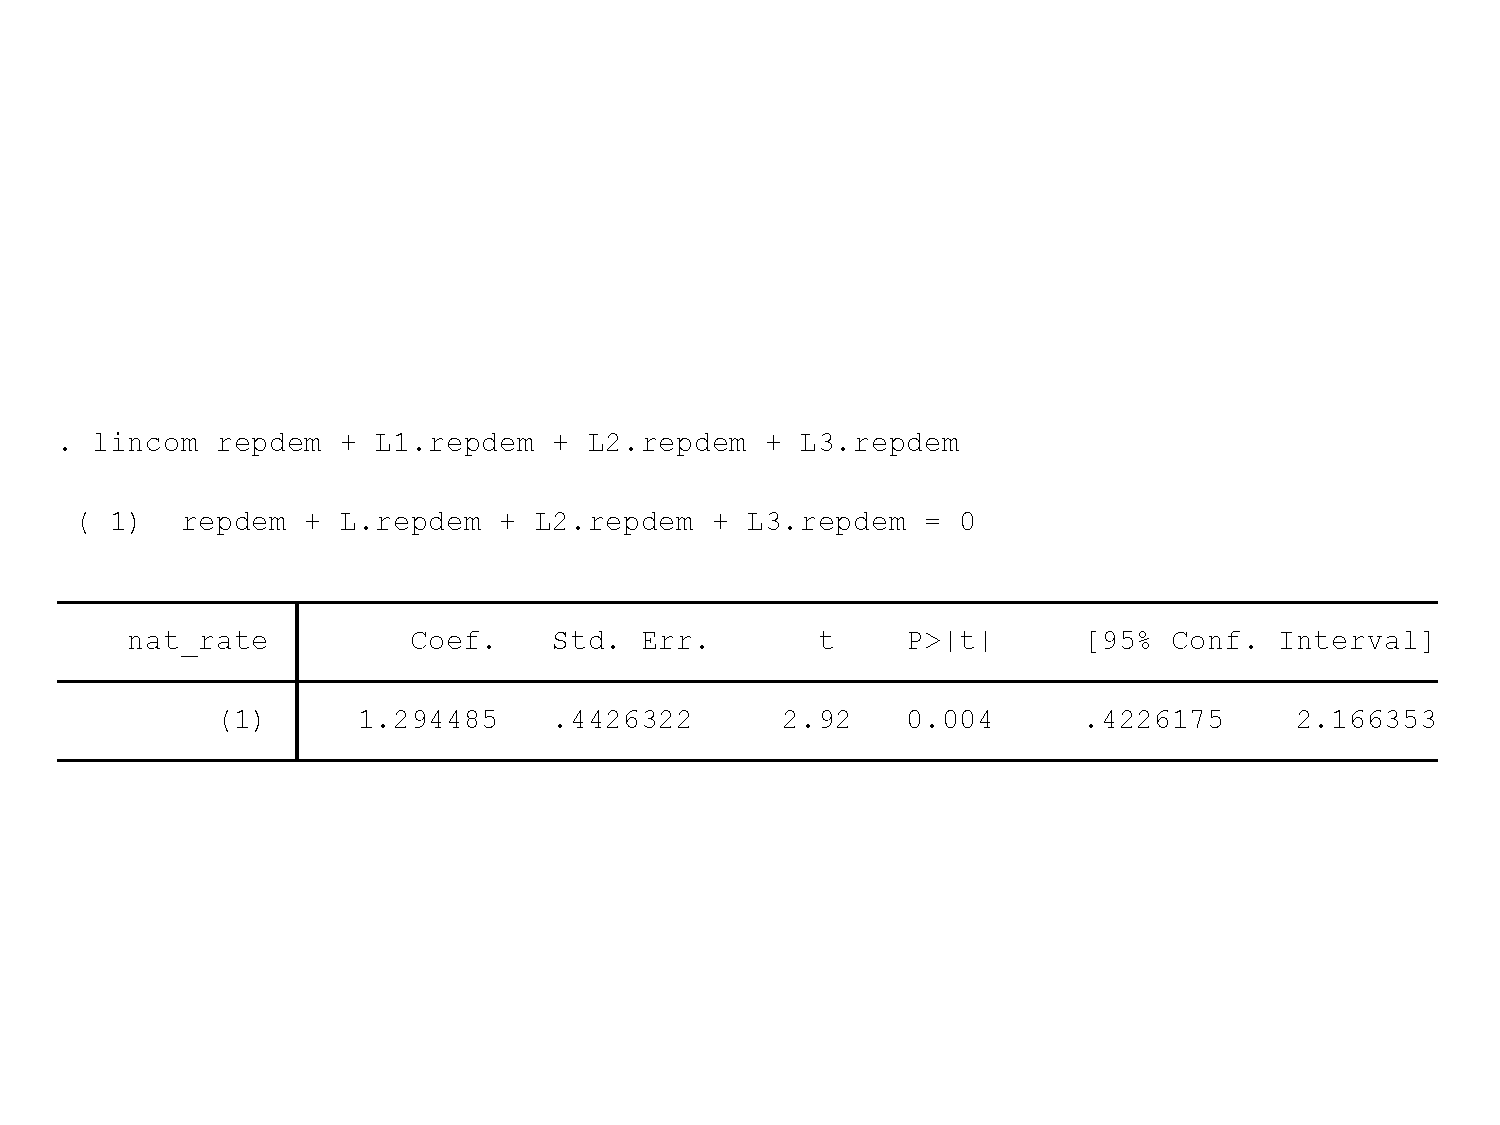
\includegraphics[height=1.4in,keepaspectratio=1]{FDL2.pdf}
\end{center}
\end{frame}
\fi

\begin{frame}
  \frametitle{Lags and Leads Model}
\vspace{-.2in}
\[
y_{it} = x_{it+1}\b_{-1} + x_{it}\b_0 + x_{it-1}\b_1 + x_{it-2}\b_2+ c_i + \varepsilon_{it}, \quad \quad t=1,2,...,T
\]\vspace{-.1in}
\begin{itemize}
    \item Can use estimate of $\b_{-1}$ to test for anticipation effects
      \begin{itemize}
      \item Consider \alert{temporary increase} in $x_{it}$ from level $m$ to $m+1$ at $t$
      \begin{itemize}
        \item $y_{t-2}= \b_{-1} m +  m \b_0 + m \b_1 + m \b_2+ c_i$
        \item $y_{t-1}= \b_{-1} \alert{(m+1)} +  m \b_0 + m \b_1 + m \b_2+ c_i$
      \end{itemize}
      \end{itemize}\medskip\pause
  \item Anticipation effect: $\b_{-1}=y_{t-1}-y_{t-2}$ change in $y$ in period $t-1$, the period before the temporary one-unit increase in $x$\medskip\pause
\item Placebo test: if $x$ causes $y$, but $y$ does not cause $x$, then $\b_{-1}$ should be close to zero
\end{itemize}
\end{frame}

\if\solutions1
\begin{frame}
  \frametitle{Leads and Lags}
\begin{center}
  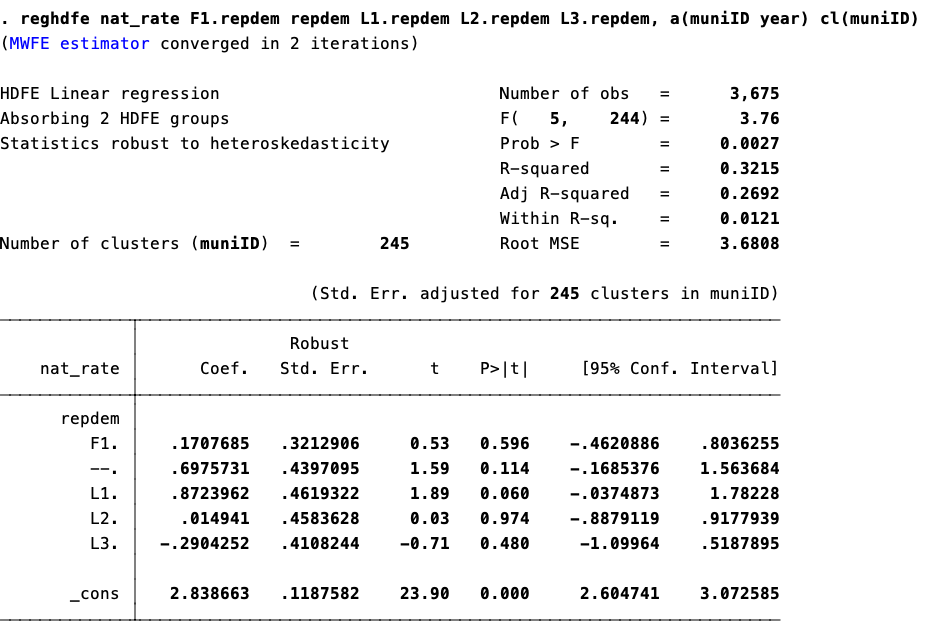
\includegraphics[height=2.7in,keepaspectratio=1]{FDL2a.png}
\end{center}
\end{frame}
\fi


% \footnotesize

% \begin{verbatim}
% > d <- ddply( 
% +   d, .(muniID), transform,
% +   lead_repdem = c( repdem[-1],NA ) 
% + )
% > d <- plm.data(d, indexes = c("muniID", "year"))
% > mod_lagleads    <- plm(nat_rate~lead_repdem+
% repdem+lag(repdem,1)+lag(repdem,2)+lag(repdem,3)+
% +                     year,data=d,model="within")
% > coeftest(mod_lagleads, vcov=function(x) 
% vcovHC(x, cluster="group", type="HC1"))

% t test of coefficients:

%                 Estimate Std. Error t value  Pr(>|t|)    
% lead_repdem     0.170768   0.320634  0.5326 0.5943479    
% repdem          0.697573   0.438811  1.5897 0.1119975    
% lag(repdem, 1)  0.872396   0.460988  1.8924 0.0585159 .  
% lag(repdem, 2)  0.014941   0.457426  0.0327 0.9739451    
% lag(repdem, 3) -0.290425   0.409985 -0.7084 0.4787574    
% year1995        0.032882   0.204374  0.1609 0.8721896    


\begin{frame}
  \frametitle{The Autor Test}
\begin{itemize}
%\item Let $S_{it}$ be a binary treatment indicator coded $1$ if unit $i$ is in treatment condition and $0$ if in control condition at $t$
\item Let $D_{it}$ be a binary indicator coded 1 if unit $i$ \alert{switched} from control to treatment between $t$ and $t-1$; 0 otherwise
    \begin{itemize}
      \item Lags: $D_{it-1}$: unit switched between $t-1$ and $t-2$
      \item Leads: $D_{it+1}$: unit switches between $t+1$ and $t$
    \end{itemize}\medskip\pause
\item Include lags and leads into the fixed effects model:
\[
y_{it} = D_{i\alert{t+2}}\b_{-2} + D_{i\alert{t+1}}\b_{-1}  + D_{i\alert{t}}\b_0 + D_{i\alert{t-1}}\b_1 + D_{i\alert{t-2}}\b_2+ c_i + \varepsilon_{it}
\]\vspace{-.2in}\medskip\pause
\item Interpretation of coefficients:
    \begin{itemize}
    \item Leads $\b_{-1}$, $\b_{-2}$, etc. test for anticipation effects
    \item Switch $\b_{0}$ tests for immediate effect
    \item Lags $\b_{1}$, $\b_{2}$, etc. test for long-run effects
    \begin{itemize}
      \item  highest lag dummy can be coded 1 for all post-switch years
    \end{itemize}
\end{itemize}
\end{itemize}
\end{frame}


% \footnotesize
% \begin{verbatim}
% > mod_all    <- plm(nat_rate~lag3+lag2+lag1+switcht+
% lead1+lead2+lead3+lead4+lead5+
% +                          year,data=d,model="within")
% > coeftest(mod_all, vcov=function(x) 
% vcovHC(x, cluster="group", type="HC1"))

% t test of coefficients:

%           Estimate Std. Error t value  Pr(>|t|)    
% lag3      1.160345   0.506989  2.2887 0.0221442 *  
% lag2      1.743682   0.538419  3.2385 0.0012105 ** 
% lag1      1.881663   0.487013  3.8637 0.0001133 ***
% switcht   0.756479   0.427751  1.7685 0.0770463 .  
% lead1     0.213876   0.389191  0.5495 0.5826635    
% lead2     0.084368   0.356799  0.2365 0.8130891    
% lead3     0.144045   0.318756  0.4519 0.6513661    
% lead4     0.075019   0.298425  0.2514 0.8015287    
% lead5    -0.094241   0.259448 -0.3632 0.7164439    
% year1992  0.385289   0.172172  2.2378 0.0252829 *  
% \end{verbatim}


\begin{frame}
  \frametitle{Dynamic Effect of Switching to Representative Democracy}
\begin{center}
  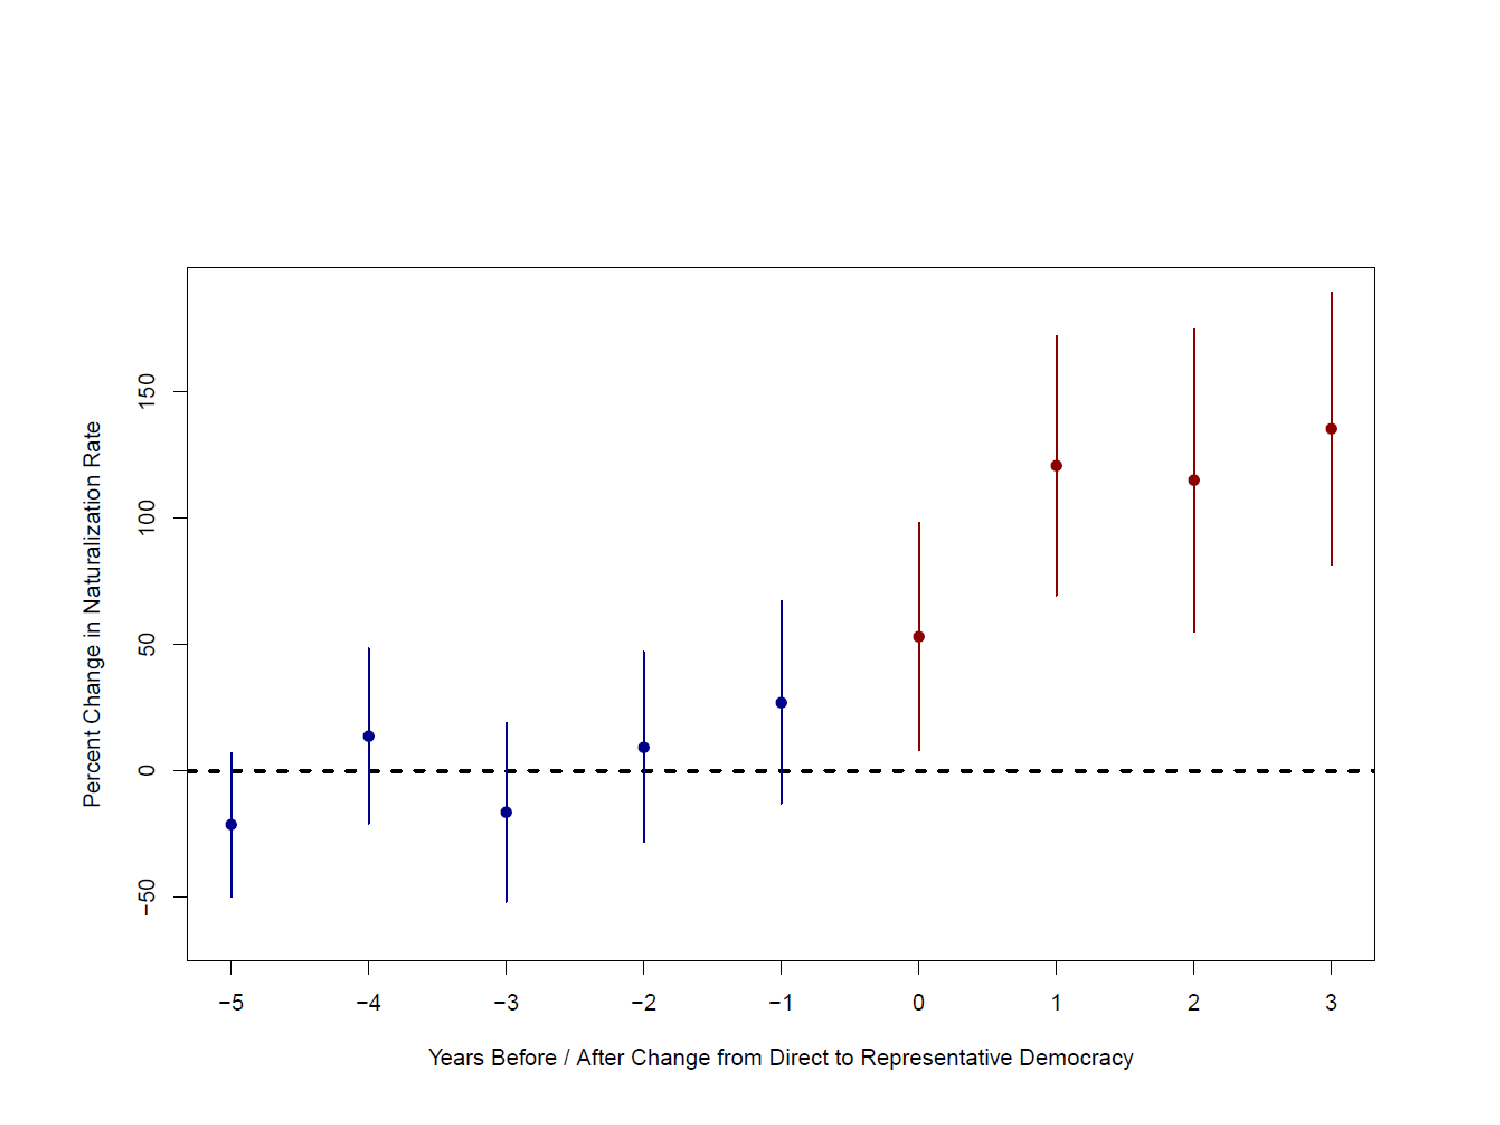
\includegraphics[height=2.8in,keepaspectratio=1]{autor3.pdf}
\end{center}
\end{frame}


\begin{frame}
  \frametitle{Lagged Dependent Variables (LDVs)}
\begin{columns}
\column{.65\textwidth}  
\vspace{-.2in}
\[
y_{it} =  \alpha\, y_{it-1} + c_i + \varepsilon_{it}, \quad \quad t=1,2,...,T
\]\vspace{-.2in}
\begin{itemize}[<+->]\itemsep0.3em\small
\item $y_{it}$ could be capital stock of firm $i$ at time $t$, and $\alpha$ the capital depreciation rate
\item Models with unit fixed effects and lagged $y$ do not produce consistent estimators (\alert{Nickell bias})
\begin{itemize}
  \item after taking first differences to eliminate $c_i$, the differenced residual $\Delta \varepsilon_{it}$ is correlated with the lagged dependent variable $\Delta y_{it-1}$ by construction
\end{itemize}
\item We might use past levels $y_{it-2}$ as an instrument for $\Delta y_{it-1}$ and apply a general method of moment (GMM) estimator, but this requires strong assumptions (e.g. no serial correlation in $\varepsilon_{it}$)
\item When $T \rightarrow \infty$, the Nickell bias goes to 0; controlling for LDVs is fine as long as they are not correlated with treatment assignment
\item However, many existing studies do not survive adding one LDV
\end{itemize}
\column{.35\textwidth}\centering
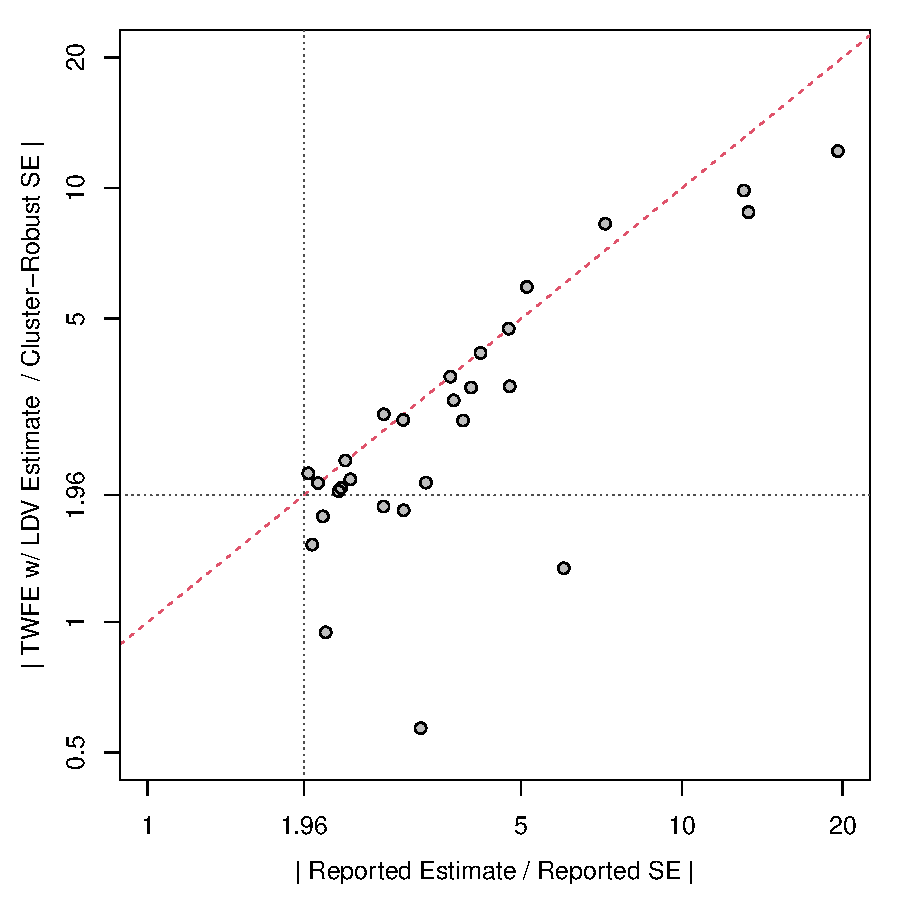
\includegraphics[width = \textwidth]{alter_twfe_ldv.pdf}
\end{columns}
\end{frame}


\begin{frame}
  \frametitle{Heterogeneous Treatment Effects}
  \small
\begin{itemize}[<+->]
  \item So far we have assumed that the treatment effect is constant across units
  \item We can allow for heterogeneous treatment effects by including interaction of treatment with other regressors
  \[
  y_{it} = treat_{it}\alpha_0 + (treat_{it}\cdot x_{it} )\alpha_1 + x_{it}\b  + c_i + t +  \varepsilon_{it}, \quad \quad t=1,2,...,T
  \]
\item Often the treatment is interacted with a time-invariant regressor:
    \[
      y_{it} = treat_{it}\alpha_0 + (treat_{it} \cdot x_{i} )\alpha_1 + c_i + t +  \varepsilon_{it}, \quad \quad t=1,2,...,T
    \]\vspace{-.1in}
    \begin{itemize}
      \item Note: The lower order term on the time-invariant $x_{i}$ is collinear with the fixed effects and drops out
    \end{itemize}
%\item For panel analysis in a fully heterogenous treatment effects framework see Imai and Kim (2012, Mimeo Princeton)
\end{itemize}

\end{frame}


\begin{frame}
  \frametitle{Heterogeneous Effect of Direct Democracy}
\begin{center}
  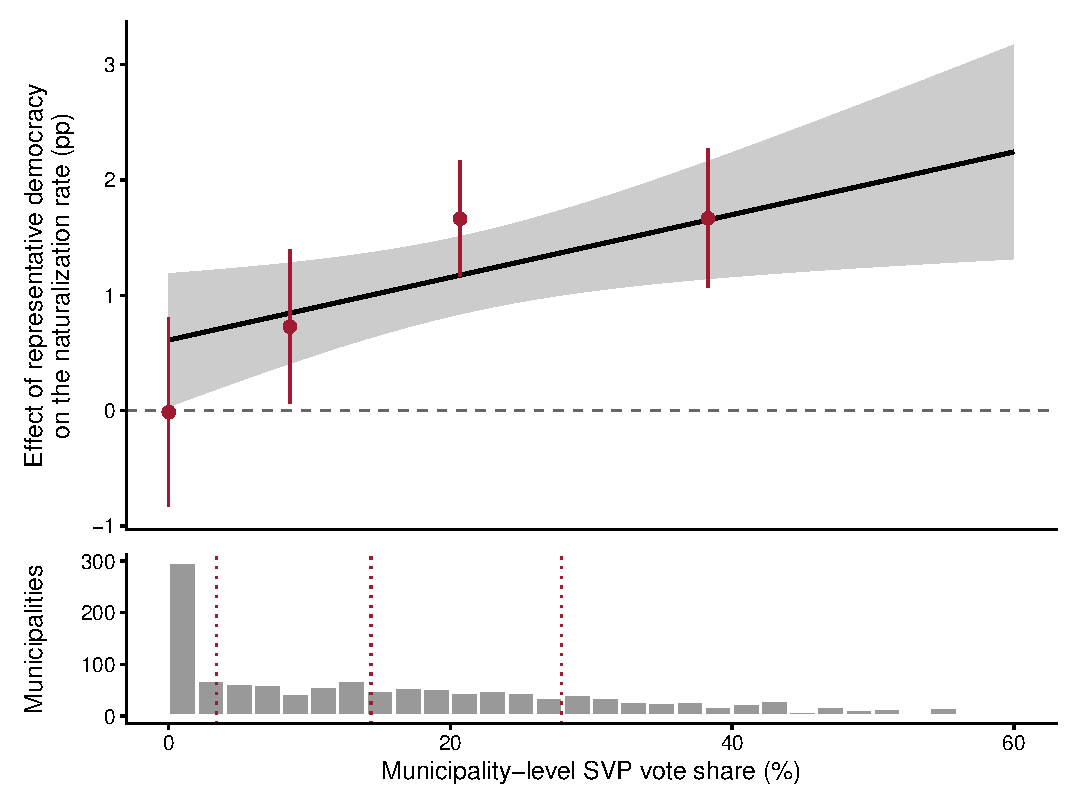
\includegraphics[height=2.55in,keepaspectratio=1]{svp_heterogeneity_2026.pdf}
\end{center}
\slidesource{Own estimates on the \textcite{hainmueller2019direct} data: two-way fixed effects with a linear interaction (line, 95\% band) and by quartile of the SVP share (points); municipality-clustered standard errors (\texttt{svp\_heterogeneity\_2026.R}).}
\end{frame}


\appendix

\setbeamertemplate{frametitle continuation}[from second][(cont.)]
\begin{frame}[t,allowframebreaks=1.0]
  \frametitle{References}
  \referencelist
  \vfill{\footnotesize\color{gray}Parts of this lecture build on teaching slides by Jens Hainmueller.}
\end{frame}

\end{document}

